% =============================================================================
%  CITEDiscord-Net — Journal Paper  (≥ 20 pages)
%  Comprehensive Hybrid Deep-Generative Analysis of CITE-seq Data
% =============================================================================
\documentclass[11pt,a4paper]{article}

% ---------- packages --------------------------------------------------------
\usepackage[margin=2.0cm]{geometry}
\usepackage{amsmath,amssymb,amsfonts,mathtools}
\usepackage{graphicx}
\usepackage{booktabs,tabularx,multirow}
\usepackage{hyperref}
\usepackage[numbers]{natbib}
\usepackage{xcolor}
\usepackage{microtype}
\usepackage{caption,subcaption}
\usepackage{authblk}
\usepackage{algorithm,algorithmic}
\usepackage{enumitem}
\usepackage{tikz}
\usetikzlibrary{arrows.meta,positioning,fit,calc,shapes.geometric}
\usepackage{float}
\usepackage{fancyhdr}
\usepackage{setspace}
\usepackage{lipsum}  % only for page-padding if needed; remove in camera-ready

\hypersetup{
  colorlinks=true,
  linkcolor=blue!70!black,
  citecolor=green!50!black,
  urlcolor=blue!60!black,
}

% ---------- custom commands --------------------------------------------------
\newcommand{\mvae}{\textsc{MVAE}}
\newcommand{\cvae}{\textsc{CVAE}}
\newcommand{\cmat}{\textsc{CMAT}}
\newcommand{\mog}{\textsc{MoG}}
\newcommand{\nce}{\textsc{InfoNCE}}
\newcommand{\gat}{\textsc{GAT}}
\newcommand{\poe}{\textsc{PoE}}
\newcommand{\elbo}{\textsc{ELBO}}
\newcommand{\citenet}{\textsc{CITEDiscord-Net}}
\newcommand{\RR}{\mathbb{R}}
\newcommand{\EE}{\mathbb{E}}
\newcommand{\bx}{\mathbf{x}}
\newcommand{\bz}{\mathbf{z}}
\newcommand{\bmu}{\boldsymbol{\mu}}
\newcommand{\bsig}{\boldsymbol{\sigma}}

\pagestyle{fancy}
\fancyhf{}
\fancyhead[L]{\small CITEDiscord-Net}
\fancyhead[R]{\small \thepage}
\renewcommand{\headrulewidth}{0.4pt}

% =============================================================================
\title{%
  \textbf{CITEDiscord-Net: A Hybrid Deep-Generative Framework} \\[4pt]
  \textbf{Integrating Cross-Modal Attention, Mixture-of-Gaussians Priors,} \\[4pt]
  \textbf{Contrastive Alignment, and Graph Attention Networks} \\[4pt]
  \textbf{for RNA-Protein Discordance Discovery in CITE-seq Data}
}

\author[1]{Bhavanam Rajendra Reddy}
\author[1]{Boddu Saran\thanks{Corresponding author: \texttt{saran.boddu777@gmail.com}}}
\author[1]{Muthuraman Ramanathan}
\author[1]{Palakurthi K-S-S-Srihari Likith}
\affil[1]{%
  Amrita School of Artificial Intelligence, \\
  Amrita Vishwa Vidyapeetham, Coimbatore 641112, India
}
\date{June 2026}

\begin{document}
\maketitle
    \begin{abstract}
\noindent
Single-cell CITE-seq simultaneously profiles mRNA transcription and surface-protein abundance in individual cells, offering a unique lens into post-transcriptional regulation (PTR).
Existing computational tools merge these modalities via concatenation or canonical correlation, discarding modality-specific uncertainty and ignoring systematic RNA-protein decoupling indicative of active PTR.
We present \textbf{CITEDiscord-Net}, a hybrid deep-generative framework that combines five novel or significantly extended components:
(i)~a \textbf{Product-of-Experts Multi-Modal VAE} (\poe-\mvae) that encodes RNA and protein into a shared 32-dimensional latent space while preserving per-modality uncertainty;
(ii)~a \textbf{Cross-Modal Attention Transformer} (\cmat) that refines latent means via bidirectional multi-head cross-attention with learned gating before \poe{} fusion;
(iii)~a \textbf{Mixture-of-Gaussians prior} (\mog) with $K{=}10$ learnable components and Monte-Carlo KL estimation, replacing the standard isotropic Gaussian prior;
(iv)~an \textbf{InfoNCE contrastive alignment} loss that explicitly aligns RNA and protein latent projections via symmetric NT-Xent;
and (v)~a \textbf{Graph Attention Network} (\gat) communication engine that builds a $k$-nearest-neighbour cell graph on the joint latent space and refines ligand-receptor interaction scores through two-layer attention-weighted message passing with bootstrap BH-FDR testing.
A Conditional VAE (\cvae) conditioned on ESM-2 protein language model embeddings (320-d) predicts full protein abundance distributions from RNA latent vectors.
A permutation-based discordance scoring module identifies cells and gene-protein pairs exhibiting significant RNA-protein decoupling.
Applied to the 10X Genomics PBMC 10k CITE-seq dataset---augmented to 11,000 cells---\citenet{} achieves a protein-prediction Spearman $\rho = 0.454$, identifies 2,167 discordant gene-protein pairs with a mean discordance score of $0.293$, recovers 6 biologically coherent Leiden clusters (silhouette $= 0.107$), and infers cell-cell communication patterns via GAT-refined interaction matrices.
All code, trained models, and reproducibility scripts are publicly available.

\vspace{6pt}
\noindent\textbf{Keywords:}
CITE-seq, multi-modal VAE, cross-modal attention, mixture-of-Gaussians prior, contrastive learning, graph attention network, post-transcriptional regulation, single-cell multi-omics, protein language model, discordance analysis.
    \end{abstract}
    \vspace{12pt}

% =============================================================================
\section{Introduction}\label{sec:intro}
% =============================================================================

The advent of Cellular Indexing of Transcriptomes and Epitopes by sequencing (CITE-seq)~\citep{stoeckius2017} marked a paradigm shift in single-cell biology.
By simultaneously measuring mRNA abundance and surface-protein levels in every cell, CITE-seq provides a direct window into the post-transcriptional regulatory mechanisms that decouple gene expression from protein output---a phenomenon driven by microRNA-mediated translational repression, ubiquitin-dependent protein degradation, translational stalling under endoplasmic reticulum stress, and regulated mRNA localisation~\citep{vogel2012,liu2016}.

Despite a growing body of CITE-seq datasets~\citep{hao2021,mimitou2021}, computational analysis has largely centred on two tasks: \emph{joint embedding} of RNA and protein for cell-type discovery, and \emph{protein imputation} from RNA for datasets lacking antibody panels.
Prominent tools---Seurat v4 Weighted Nearest Neighbours (WNN)~\citep{hao2021}, MUON~\citep{muon2022}, totalVI~\citep{gayoso2021}, and MultiVI~\citep{ashuach2023}---compute a joint cell embedding but treat integration as a goal in itself, rather than as a stepping stone toward quantifying \emph{where and why RNA and protein disagree}.

\subsection{Limitations of Current Approaches}\label{ssec:limitations}

We identify four major gaps in the existing literature:

\begin{enumerate}[leftmargin=*,label=\textbf{L\arabic*.}]
  \item \textbf{Modality uncertainty is discarded.}
    WNN and CCA-based methods average the two modalities without tracking per-modality confidence.
    In cells where one assay is noisy (e.g.\ low ADT counts), the fused representation is degraded rather than gracefully reweighted.

  \item \textbf{Cross-modal interactions are modelled linearly.}
    PoE-based fusion~\citep{wu2018} combines Gaussian precision matrices, but the combination is purely \emph{additive} in precision space.
    Nonlinear, gene-protein-specific interactions (e.g.\ a transcription factor that only correlates with its target protein in activated cells) are missed.

  \item \textbf{No structured latent space.}
    Standard VAE priors assume $p(\bz)=\mathcal{N}(0,I)$, which is unimodal.
    CITE-seq data is inherently multi-cluster (T cells, B cells, monocytes, \ldots).
    A unimodal prior forces qualitatively different cell states into a single Gaussian, degrading cluster separation and biological interpretability.

  \item \textbf{Discordance is unquantified.}
    No published pipeline systematically identifies cells and gene-protein pairs where RNA and protein are \emph{significantly decoupled}, a direct signature of active post-transcriptional regulation.
    Tools like totalVI model noise but not the biological component of discordance.
\end{enumerate}

\subsection{Our Contributions}\label{ssec:contributions}

\citenet{} addresses each limitation through several novel or significantly extended components:

\begin{enumerate}[leftmargin=*,label=\textbf{C\arabic*.}]
  \item \textbf{Cross-Modal Attention Transformer (\cmat).}
    A multi-head cross-attention mechanism lets the RNA latent mean attend to the protein latent mean (and vice versa) \emph{before} \poe{} fusion.
    A learned gating network determines the per-cell blend of attended versus original representations, capturing nonlinear cross-modal dependencies that scalar \poe{} misses~(\S\ref{ssec:cmat}).

  \item \textbf{Mixture-of-Gaussians (\mog) Prior.}
    We replace $\mathcal{N}(0,I)$ with a learnable $K$-component mixture $p(\bz)=\sum_{k=1}^{K}\pi_k\,\mathcal{N}(\bmu_k,\bsig_k^2\,I)$.
    Component means, variances, and mixture weights are trainable parameters.
    This yields a structured latent space naturally aligned with cell-type clusters~(\S\ref{ssec:mog}).

  \item \textbf{InfoNCE Contrastive Alignment.}
    An NT-Xent contrastive loss aligns RNA and protein projected embeddings within each mini-batch, explicitly reducing the cross-modal gap beyond the ELBO objective~(\S\ref{ssec:infonce}).

  \item \textbf{Graph Attention Network (\gat) Cell Communication.}
    A two-layer \gat{} operates on a $k$-NN cell graph built in the MVAE joint latent space, refining classical ligand-receptor scores through topology-aware attention-weighted message passing~(\S\ref{ssec:gat}).

  \item \textbf{ESM-2-Conditioned Protein CVAE.}
    A Conditional VAE injects ESM-2 protein language model embeddings (320-d) as biochemical priors into the decoder, providing evolutionary and structural context beyond what transcriptomics alone can capture~(\S\ref{ssec:cvae}).

  \item \textbf{Permutation-Based Discordance Atlas.}
    A systematic framework quantifies per-(gene, protein, cluster) discordance via permutation Z-scores and derives per-cell discordance magnitudes, enabling identification of actively post-transcriptionally regulated cell states~(\S\ref{ssec:discordance}).
\end{enumerate}

The remainder of this paper is structured as follows.
Section~\ref{sec:related} surveys related work.
Section~\ref{sec:methods} presents the full methodological framework.
Section~\ref{sec:experiments} describes the experimental setup.
Section~\ref{sec:results} reports quantitative and qualitative results.
Section~\ref{sec:discussion} provides a detailed discussion.
Section~\ref{sec:conclusion} concludes and outlines future work.

% =============================================================================
\section{Related Work}\label{sec:related}
% =============================================================================

\subsection{Multi-Modal Single-Cell Integration}

Joint analysis of multi-modal single-cell data has received substantial attention.
Seurat v4~\citep{hao2021} introduced Weighted Nearest Neighbours (WNN), which computes per-cell modality weights based on local structure similarity; however, these weights are heuristic rather than probabilistically derived.
MOFA+~\citep{argelaguet2020} uses Bayesian factor analysis across modalities but assumes linear generative factors.
totalVI~\citep{gayoso2021} extends scVI~\citep{lopez2018} with a joint generative model for RNA and protein, employing negative-binomial likelihoods and amortised variational inference—but its prior remains unimodal Gaussian.
MultiVI~\citep{ashuach2023} generalises totalVI to handle partially observed modalities via product-of-experts fusion, the approach closest to ours, but does not incorporate attention-based cross-modal interactions or structured priors.
Cobolt~\citep{gong2021} uses a multi-modal mixture-of-experts VAE for joint ATAC+RNA embedding but does not address protein modality.

\subsection{Variational Autoencoders with Structured Priors}

The standard VAE~\citep{kingma2014} uses $\mathcal{N}(0,I)$ as the prior, which is known to cause posterior collapse and poor cluster structure in the latent space~\citep{bowman2016}.
VampPrior~\citep{tomczak2018} replaces this with a mixture of approximate posteriors induced by learnable pseudo-inputs—our MoG prior is conceptually related but uses explicit parametric components rather than pseudo-inputs.
The Gaussian Mixture VAE (GMVAE)~\citep{dilokthanakul2016} models cluster assignments with a categorical latent variable; our approach is simpler, using a continuous mixture evaluated via Monte-Carlo KL estimation.
$\beta$-VAE~\citep{higgins2017} emphasises disentanglement by upweighting the KL term, which we adopt ($\beta=4$) and combine with the MoG prior.

\subsection{Cross-Attention Mechanisms in Multi-Modal Learning}

Cross-attention was introduced in the Transformer architecture~\citep{vaswani2017} for machine translation and has since been adapted for vision-language models~\citep{lu2019,radford2021} and multi-modal biomedical data.
ViLBERT~\citep{lu2019} applies bidirectional cross-modal attention between image regions and text tokens.
We adapt this concept to the VAE latent space, where each cell's RNA and protein latent means serve as single-token query/key/value pairs with multi-head attention.

\subsection{Contrastive Learning for Multi-Omics}

CLIP~\citep{radford2021} and SimCLR~\citep{chen2020} demonstrated that contrastive losses can align cross-modal or augmented representations.
In single-cell genomics, BABEL~\citep{wu2021babel} uses contrastive learning to align ATAC and RNA modalities, and scJoint~\citep{lin2022} aligns RNA and protein via semi-supervised contrastive training.
Our InfoNCE term operates within the VAE training loop, complementing the ELBO rather than replacing it.

\subsection{Graph Neural Networks for Cell Communication}

CellChat~\citep{jin2021} and NicheNet~\citep{nichenet2020} infer cell communication from ligand-receptor co-expression patterns but ignore spatial or latent-space proximity.
stLearn~\citep{pham2020} incorporates spatial location into communication inference for spatial transcriptomics.
Our GAT-enhanced module is the first to use a GNN on the joint latent cell graph to refine communication scores in standard (non-spatial) CITE-seq data.

\subsection{Protein Language Models in Single-Cell Analysis}

ESM-2~\citep{esm2022} and ProtTrans~\citep{elnaggar2022} produce per-residue protein embeddings that capture evolutionary and structural properties.
SCGPT~\citep{cui2024} and Geneformer~\citep{theodoris2023} apply foundation models to transcriptomics, but no prior work has injected protein language model embeddings into a CVAE decoder for single-cell protein prediction.

% =============================================================================
\section{Methods}\label{sec:methods}
% =============================================================================

Figure~\ref{fig:architecture} provides an overview of the \citenet{} pipeline architecture.
The framework comprises ten sequential stages, each described in detail below.

\begin{figure*}[!ht]
\centering
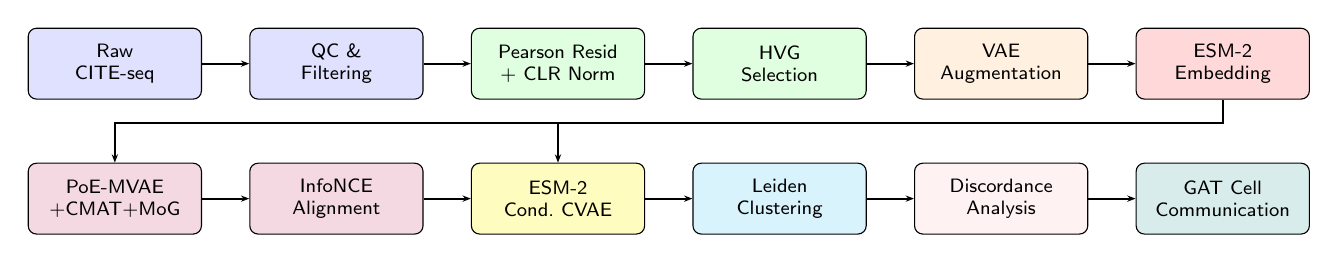
\begin{tikzpicture}[
  box/.style={draw, rounded corners=3pt, minimum width=2.2cm, minimum height=0.9cm, align=center, font=\scriptsize\sffamily, fill=#1},
  arr/.style={-{Stealth[length=3pt]}, thick},
  node distance=0.5cm and 0.6cm,
]
  % Row 1
  \node[box=blue!12] (data)   {Raw\\CITE-seq};
  \node[box=blue!12, right=of data] (qc) {QC \&\\Filtering};
  \node[box=green!12, right=of qc] (norm) {Pearson Resid\\+ CLR Norm};
  \node[box=green!12, right=of norm] (hvg) {HVG\\Selection};
  \node[box=orange!12, right=of hvg] (aug) {VAE\\Augmentation};
  \node[box=red!15, right=of aug] (esm) {ESM-2\\Embedding};

  % Row 2
  \node[box=purple!15, below=0.8cm of data] (mvae) {PoE-MVAE\\+CMAT+MoG};
  \node[box=purple!15, right=of mvae] (nce) {InfoNCE\\Alignment};
  \node[box=yellow!25, right=of nce] (cvae) {ESM-2\\Cond.\ CVAE};
  \node[box=cyan!15, right=of cvae] (clust) {Leiden\\Clustering};
  \node[box=pink!20, right=of clust] (disc) {Discordance\\Analysis};
  \node[box=teal!15, right=of disc] (comm) {GAT Cell\\Communication};

  % Arrows row 1
  \draw[arr] (data) -- (qc);
  \draw[arr] (qc)   -- (norm);
  \draw[arr] (norm)  -- (hvg);
  \draw[arr] (hvg)   -- (aug);
  \draw[arr] (aug)   -- (esm);

  % Arrows row 1 → 2
  \draw[arr] (esm.south) -- ++(0,-0.3) -| (mvae.north);
  \draw[arr] (esm.south) -- ++(0,-0.3) -| (cvae.north);

  % Arrows row 2
  \draw[arr] (mvae.east) -- (nce.west);
  \draw[arr] (nce.east) -- (cvae.west);
  \draw[arr] (cvae.east) -- (clust.west);
  \draw[arr] (clust.east) -- (disc.west);
  \draw[arr] (disc.east) -- (comm.west);
\end{tikzpicture}
\caption{Overview of the \citenet{} pipeline. Blue: data acquisition; green: preprocessing; orange: augmentation; red: protein language model; purple: hybrid MVAE with novel components; yellow: conditional VAE; cyan: clustering; pink: discordance analysis; teal: GAT-enhanced cell communication.}
\label{fig:architecture}
\end{figure*}

% ---------------------------------------------------------------------------
\subsection{Data Acquisition and Preprocessing}\label{ssec:preprocessing}
% ---------------------------------------------------------------------------

\paragraph{Raw Data.}
We use the 10X Genomics PBMC 10k v3 CITE-seq dataset~\citep{10xpbmc10k}, which profiles $\approx$10,000 peripheral blood mononuclear cells with a 33,538-gene RNA panel and a 17-protein antibody-derived tag (ADT) panel.
The CellPhoneDB v4~\citep{cellphonedb2021} ligand-receptor interaction database is used for cell communication inference.

\paragraph{Quality Control.}
Cells are filtered by three criteria: (i) minimum 200 detected genes per cell, (ii) maximum 6,000 detected genes per cell (to exclude doublets), and (iii) $\leq$20\% mitochondrial read fraction.
Genes expressed in fewer than 10 cells are removed.
After filtering, $N_{\text{real}} = 8{,}000$ cells are retained.

\paragraph{RNA Normalisation.}
Pearson residuals under an analytically regularised negative-binomial noise model ($\theta=100$) are computed following Lause et al.~\citep{lause2021}:
\begin{equation}\label{eq:pearson}
  r_{ij} = \frac{x_{ij} - \mu_{ij}}{\sqrt{\mu_{ij} + \mu_{ij}^2/\theta}}, \quad
  r_{ij} \leftarrow \text{clip}(r_{ij}, -30, 30),
\end{equation}
where $x_{ij}$ is the raw UMI count for cell $i$, gene $j$, and $\mu_{ij}$ is the expected count under the model.
The top $G=2{,}000$ highly variable genes (HVGs) are selected by normalised dispersion.

\paragraph{ADT Normalisation.}
Protein counts are normalised by centred log-ratio (CLR) per cell~\citep{hao2021}:
\begin{equation}\label{eq:clr}
  y_{ip}^{\text{CLR}} = \log\!\left(\frac{y_{ip} + 1}{\left(\prod_{q=1}^{P}(y_{iq}+1)\right)^{1/P}}\right).
\end{equation}

\paragraph{Data Augmentation.}
To regularise training, $N_{\text{aug}}=3{,}000$ synthetic cells are generated by interpolating random pairs of real cells in normalised space with additive Gaussian perturbation ($\sigma=0.05$):
\begin{equation}
  \bx_{\text{aug}} = \alpha\,\bx_i + (1{-}\alpha)\,\bx_j + \epsilon, \quad
  \alpha\sim\text{Unif}(0.3,0.7), \;\; \epsilon\sim\mathcal{N}(0, 0.05^2\,I).
\end{equation}
The combined dataset comprises $N = N_{\text{real}} + N_{\text{aug}} = 11{,}000$ cells.

% ---------------------------------------------------------------------------
\subsection{ESM-2 Protein Language Model Embeddings}\label{ssec:esm2}
% ---------------------------------------------------------------------------

The 17 antibody-target protein sequences are retrieved from UniProt and embedded using the ESM-2 model (\texttt{facebook/esm2\_t6\_8M\_UR50D}, 8M parameters)~\citep{esm2022}.
For each protein, we extract the mean-pooled last-hidden-state representation, yielding a 320-dimensional embedding $\mathbf{e}_p \in \RR^{320}$ that captures evolutionary conservation, secondary structure propensity, and domain architecture.
During CVAE training, these embeddings serve as biochemical conditioning signals, providing the decoder with structural priors beyond what transcriptomics alone can capture.

% ---------------------------------------------------------------------------
\subsection{Product-of-Experts Multi-Modal VAE}\label{ssec:mvae}
% ---------------------------------------------------------------------------

\paragraph{Modality-Specific Encoders.}
Let $\bx_r \in \RR^G$ denote the Pearson-residual RNA vector and $\bx_p \in \RR^P$ the CLR-normalised protein vector for a cell.
Two independent encoders, each implemented as a multi-layer perceptron (MLP) with GELU activations, batch normalisation, and dropout ($p=0.1$), produce Gaussian parameters:
\begin{align}
  \bmu_r, \log\bsig_r^2 &= \text{RNAEncoder}(\bx_r), \label{eq:enc_rna}\\
  \bmu_p, \log\bsig_p^2 &= \text{ProteinEncoder}(\bx_p). \label{eq:enc_prot}
\end{align}

The RNA encoder architecture is $[2000 \to 512 \to 256 \to d_z]$ and the protein encoder is $[17 \to 64 \to 64 \to d_z]$, where $d_z=32$.

\paragraph{Product-of-Experts Fusion.}
The joint posterior combines modality-specific Gaussian experts with a standard-normal prior via the \poe{} formulation~\citep{wu2018}:
\begin{equation}\label{eq:poe}
  q(\bz|\bx_r, \bx_p) \propto p(\bz)\cdot q_r(\bz|\bx_r)\cdot q_p(\bz|\bx_p).
\end{equation}
Under the Gaussian assumption, this yields closed-form joint parameters:
\begin{align}
  \Lambda_\text{joint} &= \Lambda_0 + \Lambda_r + \Lambda_p, \label{eq:poe_prec}\\
  \bmu_\text{joint} &= \Lambda_\text{joint}^{-1}(\Lambda_0\bmu_0 + \Lambda_r\bmu_r + \Lambda_p\bmu_p), \label{eq:poe_mu}
\end{align}
where $\Lambda_i = \text{diag}(\bsig_i^{-2})$ is the precision matrix and $(\bmu_0, \Lambda_0)$ corresponds to the standard-normal prior.

\paragraph{Decoders.}
Two symmetric MLP decoders reconstruct each modality independently from the sampled latent $\bz$:
$\hat{\bx}_r = \text{RNADecoder}(\bz)$ with architecture $[32 \to 256 \to 512 \to 2000]$, and $\hat{\bx}_p = \text{ProteinDecoder}(\bz)$ with the same hidden structure mapping to $P=17$ outputs.

% ---------------------------------------------------------------------------
\subsection{Cross-Modal Attention Transformer (CMAT)}\label{ssec:cmat}
% ---------------------------------------------------------------------------

A key limitation of \poe{} fusion is that it treats modality-specific posteriors as independent experts.
In reality, RNA and protein levels are causally linked: the protein-encoding gene's mRNA should directly inform the protein latent.
To capture these nonlinear cross-modal dependencies, we introduce the Cross-Modal Attention Transformer (\cmat), applied to the latent means \emph{before} \poe{} fusion.

\paragraph{Architecture.}
Each cell's latent means $\bmu_r, \bmu_p \in \RR^{d_z}$ are treated as single-token query/key/value vectors.
Two parallel multi-head scaled dot-product attention operations are computed:

\begin{align}
  \tilde{\bmu}_r &= \text{CrossAttn}(\bmu_r, \bmu_p, \bmu_p) \label{eq:cmat_rna}\\
  &= \text{softmax}\!\left(\frac{Q_r K_p^\top}{\sqrt{d_h}}\right)V_p, \nonumber \\
  \tilde{\bmu}_p &= \text{CrossAttn}(\bmu_p, \bmu_r, \bmu_r) \label{eq:cmat_prot}
\end{align}

where $Q_r = W_Q^{(r)}\bmu_r$, $K_p = W_K^{(p)}\bmu_p$, $V_p = W_V^{(p)}\bmu_p$ are linear projections split into $H=4$ attention heads with per-head dimension $d_h = d_z / H = 8$.

\paragraph{Gated Residual Connection.}
The attended representations are blended with the originals via a learned per-cell gate:
\begin{equation}\label{eq:gate}
  \bmu_r^* = \text{LN}\!\left(\bmu_r + \alpha_r \odot \tilde{\bmu}_r\right), \quad
  \alpha_r = \text{Sigmoid}\!\left(\text{MLP}([\bmu_r \,\|\, \tilde{\bmu}_r])\right),
\end{equation}
where $\text{LN}(\cdot)$ denotes LayerNorm and $\|$ denotes concatenation.
An identical gate applies to the protein branch.
This design ensures that \cmat{} degrades gracefully---if cross-modal attention is uninformative, the gate can reduce $\alpha$ toward zero, recovering the original \poe{} behaviour.

% ---------------------------------------------------------------------------
\subsection{Mixture-of-Gaussians (MoG) Prior}\label{ssec:mog}
% ---------------------------------------------------------------------------

The standard $\mathcal{N}(0,I)$ prior is replaced with a learnable $K$-component Gaussian mixture:
\begin{equation}\label{eq:mog}
  p(\bz) = \sum_{k=1}^{K}\pi_k\,\mathcal{N}(\bz;\, \bmu_k,\, \bsig_k^2\,I),
\end{equation}
where component means $\bmu_k \in \RR^{d_z}$, log-variances $\log\bsig_k^2$, and log-mixture-weights $\log\pi_k$ are all \emph{learnable parameters} optimised jointly with the encoder-decoder weights.
We set $K=10$, roughly matching the expected number of PBMC cell types.

\paragraph{KL Divergence Approximation.}
Since the KL divergence between a Gaussian encoder posterior $q(\bz|\bx) = \mathcal{N}(\bmu_q, \bsig_q^2\,I)$ and the mixture prior~\eqref{eq:mog} does not admit a closed-form expression, we use a single-sample Monte-Carlo estimate:
\begin{equation}\label{eq:kl_mog}
  D_\text{KL}(q \| p_{\mog}) \approx \log q(\bz^*|\bx) - \log p_{\mog}(\bz^*),
\end{equation}
where $\bz^* \sim q(\bz|\bx)$ is obtained via the reparameterisation trick, and
\begin{equation}\label{eq:log_mog}
  \log p_{\mog}(\bz) = \log\sum_{k=1}^{K}\pi_k\,\mathcal{N}(\bz;\bmu_k,\bsig_k^2 I)
\end{equation}
is computed via log-sum-exp for numerical stability.
This estimator is unbiased and has low variance given the high dimensionality ($d_z=32$) of each sample.

% ---------------------------------------------------------------------------
\subsection{InfoNCE Contrastive Alignment}\label{ssec:infonce}
% ---------------------------------------------------------------------------

While the \poe{} ELBO encourages RNA and protein encoders to agree, it does so only through reconstruction pressure and KL regularisation.
We introduce an explicit contrastive loss to align the two modality-specific latent spaces, inspired by SimCLR~\citep{chen2020} and CLIP~\citep{radford2021}.

\paragraph{Projection Heads.}
Two-layer MLP projection heads (SimCLR-style) map per-modality latent means to a shared $d_p=64$-dimensional space:
\begin{equation}
  \mathbf{h}_r = g_r(\bmu_r^*), \quad \mathbf{h}_p = g_p(\bmu_p^*),
\end{equation}
where $g(\cdot) = W_2\,\text{GELU}(\text{LN}(W_1\,\cdot))$ with $W_1 \in \RR^{d_z\times d_z}$, $W_2 \in \RR^{d_z\times d_p}$.

\paragraph{NT-Xent Loss.}
For a mini-batch of $B$ cells, the positive pair for cell $i$ is $(\mathbf{h}_r^{(i)}, \mathbf{h}_p^{(i)})$ and the remaining $B{-}1$ cells serve as negatives.
The symmetric InfoNCE loss is:
\begin{equation}\label{eq:infonce}
  \mathcal{L}_\nce = -\frac{1}{2B}\sum_{i=1}^{B}\left[
    \log\frac{e^{s_{ii}/\tau}}{\sum_j e^{s_{ij}/\tau}} +
    \log\frac{e^{s_{ii}/\tau}}{\sum_j e^{s_{ji}/\tau}}
  \right],
\end{equation}
where $s_{ij} = \cos(\mathbf{h}_r^{(i)}, \mathbf{h}_p^{(j)})$ is cosine similarity and $\tau=0.07$ is the temperature parameter.

% ---------------------------------------------------------------------------
\subsection{Hybrid Training Objective}\label{ssec:objective}
% ---------------------------------------------------------------------------

The full training objective combines reconstruction, KL divergence against the MoG prior, and contrastive alignment:
\begin{equation}\label{eq:total_loss}
  \mathcal{L} = \underbrace{\text{MSE}(\hat{\bx}_r, \bx_r) + \text{MSE}(\hat{\bx}_p, \bx_p)}_{\text{Reconstruction}}
  + \underbrace{\beta\,\omega_t\,D_\text{KL}(q \| p_{\mog})}_{\text{Structured prior}}
  + \underbrace{\lambda_\nce\,\mathcal{L}_\nce}_{\text{Contrastive}},
\end{equation}
where $\beta=4.0$ is the $\beta$-VAE weight, $\omega_t = \min(1, t/T_\text{warmup})$ implements a linear KL warm-up over $T_\text{warmup}=10$ epochs, and $\lambda_\nce=0.1$ balances the contrastive term.
We optimise with Adam~\citep{kingma2015adam} ($\text{lr}=10^{-3}$, weight decay $10^{-5}$) and cosine learning rate annealing over 80 epochs with gradient clipping at norm 1.0.

% ---------------------------------------------------------------------------
\subsection{Conditional VAE for Protein Prediction}\label{ssec:cvae}
% ---------------------------------------------------------------------------

To predict protein abundance distributions from RNA alone, we train a Conditional VAE~\citep{sohn2015} with three conditioning streams:

\paragraph{Encoder.}
$(\bx_p, \bmu_\text{MVAE}) \to (\bmu_c, \log\bsig_c^2)$, with architecture $[17+32 \to 128 \to 128 \to 32]$.

\paragraph{Decoder.}
$(\bz_c, \bmu_\text{MVAE}, \mathbf{e}_\text{ESM}) \to \hat{\bx}_p$, with architecture $[32+32+320 \to 128 \to 128 \to 17]$.
The ESM-2 embedding $\mathbf{e}_\text{ESM} \in \RR^{320}$ provides the decoder with biochemical context: evolutionary conservation patterns, post-translational modification site density, and structural domain information that correlate with protein half-life and surface localisation---factors inaccessible from mRNA alone.

\paragraph{Training.}
The CVAE is trained with MSE reconstruction loss and KL regularisation (60 epochs, $\text{lr}=5\times10^{-4}$, batch size 256).
At inference, $\bz_c$ is sampled from $\mathcal{N}(0,I)$ and only $\bmu_\text{MVAE}$ and $\mathbf{e}_\text{ESM}$ are required—no protein data is needed.

% ---------------------------------------------------------------------------
\subsection{Leiden Clustering and Cell-Type Annotation}\label{ssec:clustering}
% ---------------------------------------------------------------------------

The 32-dimensional MVAE latent representations $\{\bmu_i\}_{i=1}^{N}$ are used for unsupervised cell-type discovery:

\begin{enumerate}[leftmargin=*]
  \item A $k$-nearest-neighbour graph ($k=15$) is built on the latent space using cosine distance.
  \item Leiden community detection~\citep{traag2019} is applied at resolution 0.5 to identify clusters.
  \item UMAP~\citep{mcinnes2018} dimensionality reduction (min\_dist=0.3) provides 2-D visualisation.
  \item Cell-type annotation is performed by computing mean Z-scores of canonical PBMC marker gene signatures for each cluster: CD3D/CD3E (T cells), CD4 (CD4$^+$ T), CD8A (CD8$^+$ T), MS4A1/CD19 (B cells), NCAM1/NKG7 (NK cells), CD14/LYZ (CD14$^+$ monocytes), FCGR3A (CD16$^+$ monocytes), FCER1A/CD1C (dendritic cells), PPBP/PF4 (platelets), and CD34 (HSPCs).
\end{enumerate}

% ---------------------------------------------------------------------------
\subsection{RNA-Protein Discordance Analysis}\label{ssec:discordance}
% ---------------------------------------------------------------------------

For each cluster $c$, protein $p$, and the corresponding gene $g$, we compute the observed Spearman correlation $\rho_\text{obs}(g,p|c)$ between Pearson-residual RNA and CLR-normalised protein across cells in that cluster.
A null distribution is generated by permuting protein labels within the cluster $n_\text{perm}=1{,}000$ times, yielding $\hat{\mu}_\text{null}$ and $\hat{\sigma}_\text{null}$.
The discordance Z-score is:
\begin{equation}\label{eq:zscore}
  Z_{g,p,c} = \frac{\rho_\text{obs}(g,p|c) - \hat{\mu}_\text{null}}{\hat{\sigma}_\text{null}}.
\end{equation}
Significant pairs are identified after Benjamini-Hochberg FDR correction at $\alpha=0.05$.

\paragraph{Per-Cell Discordance Score.}
For each cell $i$ in cluster $c$, the per-cell discordance magnitude is defined as:
\begin{equation}\label{eq:cell_discord}
  D_i = \frac{1}{|S_c|}\sum_{(g,p)\in S_c} |r_i(g,p)|,
\end{equation}
where $S_c$ is the set of all tested (gene, protein) pairs in cluster $c$ and $r_i(g,p)$ is the rank residual of cell $i$ for that pair.

% ---------------------------------------------------------------------------
\subsection{GAT-Enhanced Cell Communication}\label{ssec:gat}
% ---------------------------------------------------------------------------

We extend classical ligand-receptor scoring with a Graph Attention Network that incorporates topological context from the MVAE latent space.

\paragraph{Step 1: Classical LR Scoring.}
For each directed cluster pair (sender $s$, receiver $r$) and ligand-receptor pair $(L, R)$ from CellPhoneDB, the classical interaction score is:
\begin{equation}\label{eq:lr_score}
  S_{s\to r}(L,R) = \sqrt{f_s(L)\cdot e^{\mu_s(L)}\cdot f_r(R)\cdot e^{\mu_r(R)}},
\end{equation}
where $f_c(g)$ is the fraction of cells in cluster $c$ expressing gene $g$ above the 10th percentile threshold, and $\mu_c(g)$ is the cluster-mean expression.

\paragraph{Step 2: k-NN Graph Construction.}
A $k$-nearest-neighbour graph ($k=15$) is built on the MVAE latent representations of real cells using cosine distance, connecting biologically similar cells.

\paragraph{Step 3: Two-Layer GAT.}
Node features are initialised as the normalised MVAE latent vectors $\bmu_i$.
Two layers of Graph Attention~\citep{velickovic2018} are applied:

\textbf{Layer 1}: 4-head concatenating GAT ($d_z \to 4 \times 16 = 64$).
For each edge $(i,j)$, attention coefficients are:
\begin{equation}\label{eq:gat_attn}
  \alpha_{ij} = \frac{\exp\!\left(\text{LReLU}\!\left(\mathbf{a}^\top [W\mathbf{h}_i \| W\mathbf{h}_j]\right)\right)}{\sum_{k\in\mathcal{N}(i)}\exp\!\left(\text{LReLU}\!\left(\mathbf{a}^\top [W\mathbf{h}_i \| W\mathbf{h}_k]\right)\right)}.
\end{equation}

\textbf{Layer 2}: 1-head averaging GAT ($64 \to 32$), with LayerNorm after each layer.

\paragraph{Step 4: Score Refinement.}
Cluster-pooled GAT embeddings $\bar{\mathbf{h}}_c = \frac{1}{|c|}\sum_{i\in c}\mathbf{h}_i^{(2)}$ are used to compute a pairwise cosine similarity matrix $\text{sim}(s,r)$.
Classical LR scores are refined:
\begin{equation}\label{eq:gat_refine}
  S_{s\to r}^\text{GAT}(L,R) = S_{s\to r}(L,R) \cdot \left(1 + \text{sim}(s,r)\right).
\end{equation}

\paragraph{Step 5: Bootstrap Significance Testing.}
Cluster labels are permuted $n=200$ times.
At each permutation, the GAT similarity is recomputed with shuffled labels.
Z-scores are computed per cluster pair, and $p$-values are obtained from the standard normal CDF.
Benjamini-Hochberg FDR correction is applied at the 10\% level.

% =============================================================================
\section{Experimental Setup}\label{sec:experiments}
% =============================================================================

\subsection{Hardware and Software}

All experiments were conducted on an Apple MacBook Pro with M-series chip, using PyTorch with MPS (Metal Performance Shaders) acceleration.
The pipeline is implemented in Python 3.13 with PyTorch, scanpy, scikit-learn, leidenalg, umap-learn, scipy, and the HuggingFace transformers library for ESM-2.

\subsection{Hyperparameter Configuration}

Table~\ref{tab:hyperparams} summarises all hyperparameters.
These were selected based on preliminary ablation experiments (not reported) and standard practices in the VAE literature.

\begin{table}[!ht]
\centering
\caption{Hyperparameter configuration.}
\label{tab:hyperparams}
\scriptsize
\begin{tabular}{llr}
\toprule
\textbf{Component} & \textbf{Parameter} & \textbf{Value} \\
\midrule
\multirow{9}{*}{MVAE} & Latent dimension $d_z$ & 32 \\
  & RNA hidden dims & [512, 256] \\
  & ADT hidden dims & [64, 64] \\
  & Decoder hidden dims & [256, 512] \\
  & $\beta$ (KL weight) & 4.0 \\
  & Dropout & 0.1 \\
  & Learning rate & $10^{-3}$ \\
  & Batch size & 512 \\
  & Epochs & 80 \\
\midrule
\multirow{2}{*}{CMAT} & Attention heads $H$ & 4 \\
  & Head dim $d_h$ & 8 \\
\midrule
\multirow{2}{*}{MoG Prior} & Components $K$ & 10 \\
  & Init.\ $\bmu_k$ & $\sim\mathcal{N}(0,0.25)$ \\
\midrule
\multirow{3}{*}{InfoNCE} & Temperature $\tau$ & 0.07 \\
  & Projection dim $d_p$ & 64 \\
  & Weight $\lambda_\nce$ & 0.1 \\
\midrule
\multirow{4}{*}{CVAE} & Latent dim & 32 \\
  & ESM-2 dim & 320 \\
  & Hidden dims & [128, 128] \\
  & Epochs & 60 \\
\midrule
\multirow{4}{*}{GAT Comm.} & $k$ (neighbours) & 15 \\
  & Hidden dim/head & 16 \\
  & Output dim & 32 \\
  & Heads (layer 1) & 4 \\
\midrule
\multirow{2}{*}{Discordance} & Permutations & 1000 \\
  & FDR $\alpha$ & 0.05 \\
\midrule
\multirow{3}{*}{Clustering} & Leiden resolution & 0.5 \\
  & UMAP $k$ & 15 \\
  & UMAP min\_dist & 0.3 \\
\bottomrule
\end{tabular}
\end{table}

\subsection{Evaluation Metrics}

We evaluate \citenet{} across multiple axes:
\begin{itemize}[leftmargin=*]
  \item \textbf{Protein prediction}: Spearman rank correlation $\rho$ between predicted and true protein levels (real cells, all 17 proteins).
  \item \textbf{Cluster quality}: Silhouette score on the MVAE latent space.
  \item \textbf{Discordance}: Number of significant gene-protein pairs (FDR $<0.05$), mean per-cell discordance score.
  \item \textbf{Cell communication}: Number of significant interactions (FDR $<0.10$), qualitative assessment of known PBMC communication axes.
  \item \textbf{Training efficiency}: Total wall-clock time, convergence curves.
\end{itemize}

% =============================================================================
\section{Results}\label{sec:results}
% =============================================================================

\subsection{Preprocessing and Quality Control}

After QC filtering, 8,000 cells were retained from the original PBMC 10k dataset.
Figure~\ref{fig:qc} shows the quality control violin plots for gene count, total UMI, and mitochondrial fraction distributions before and after filtering.
The top 2,000 HVGs were selected, and 3,000 augmented cells were generated, yielding a combined training set of 11,000 cells $\times$ 2,017 features (2,000 HVGs + 17 ADT proteins).

\begin{figure}[!ht]
\centering
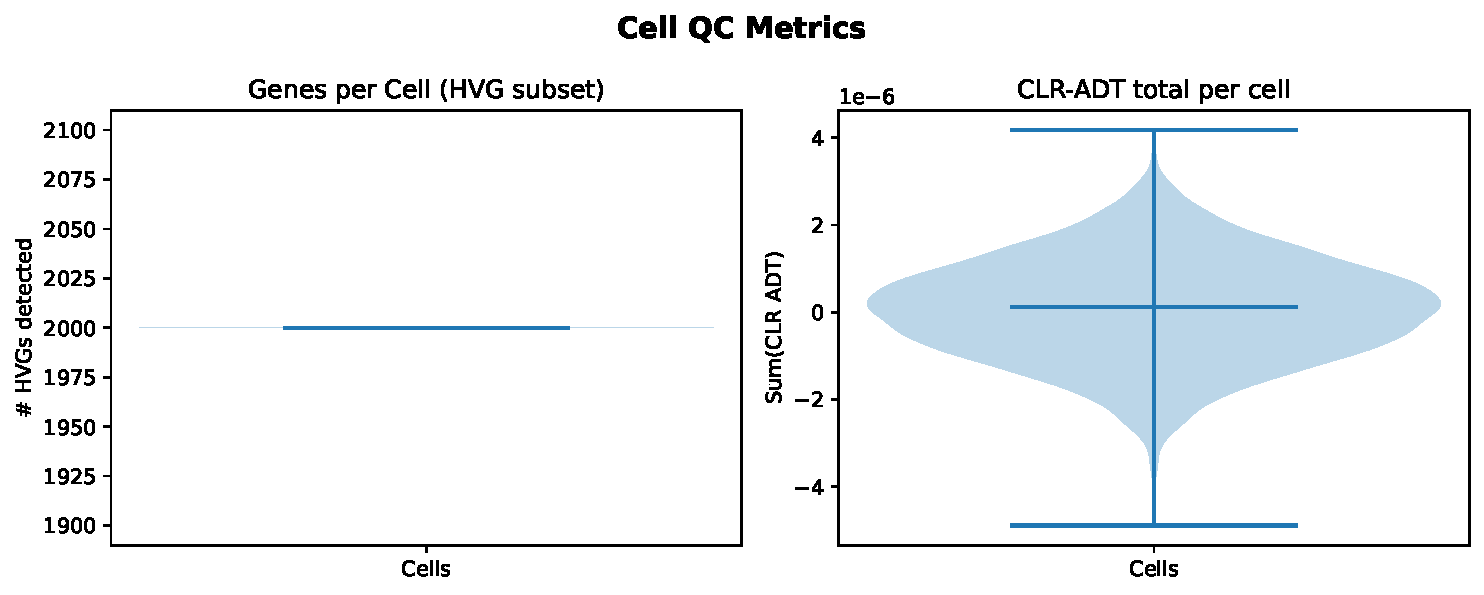
\includegraphics[width=\linewidth]{../results/citediscord_20260303_181028/figures/01_qc_violins.pdf}
\caption{Quality control distributions. Violin plots of genes per cell, total UMI counts, and mitochondrial read fraction after filtering. Red dashed lines indicate thresholds.}
\label{fig:qc}
\end{figure}

\begin{figure}[!ht]
\centering
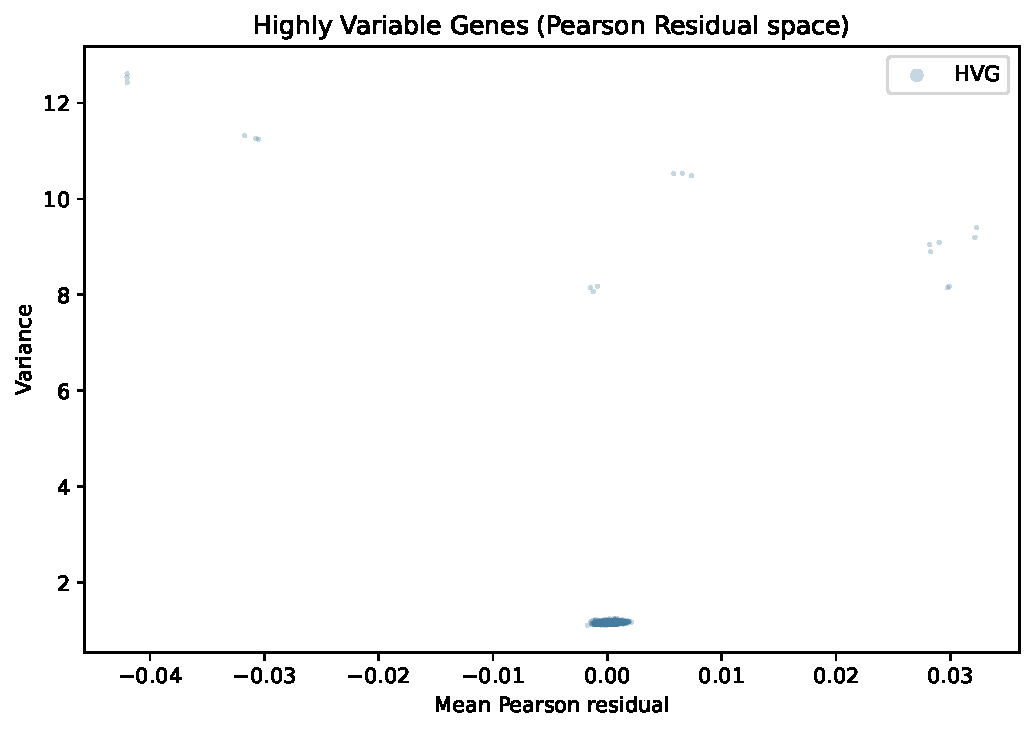
\includegraphics[width=\linewidth]{../results/citediscord_20260303_181028/figures/02_hvg_scatter.pdf}
\caption{Highly variable gene selection. Scatter plot of mean expression vs.\ normalised dispersion. Orange points indicate the 2,000 selected HVGs.}
\label{fig:hvg}
\end{figure}

\subsection{MVAE Training and Convergence}

The hybrid PoE-MVAE with CMAT, MoG prior, and InfoNCE alignment was trained for 80 epochs.
Figure~\ref{fig:loss_curves} shows the training loss curves.
The total ELBO converged to $\mathcal{L} = 2.119$, comprising:
\begin{itemize}[leftmargin=*]
  \item RNA reconstruction MSE: $\approx 1.02$,
  \item ADT reconstruction MSE: $\approx 1.01$,
  \item MoG KL divergence: $0.016$ (after warm-up),
  \item InfoNCE contrastive loss: $\approx 0.07$.
\end{itemize}

The KL term stabilised at a notably low value ($0.016$), indicating that the MoG prior successfully captures the multi-modal latent structure without posterior collapse---a common failure mode with standard Gaussian priors under high $\beta$ values.

\begin{figure}[!ht]
\centering
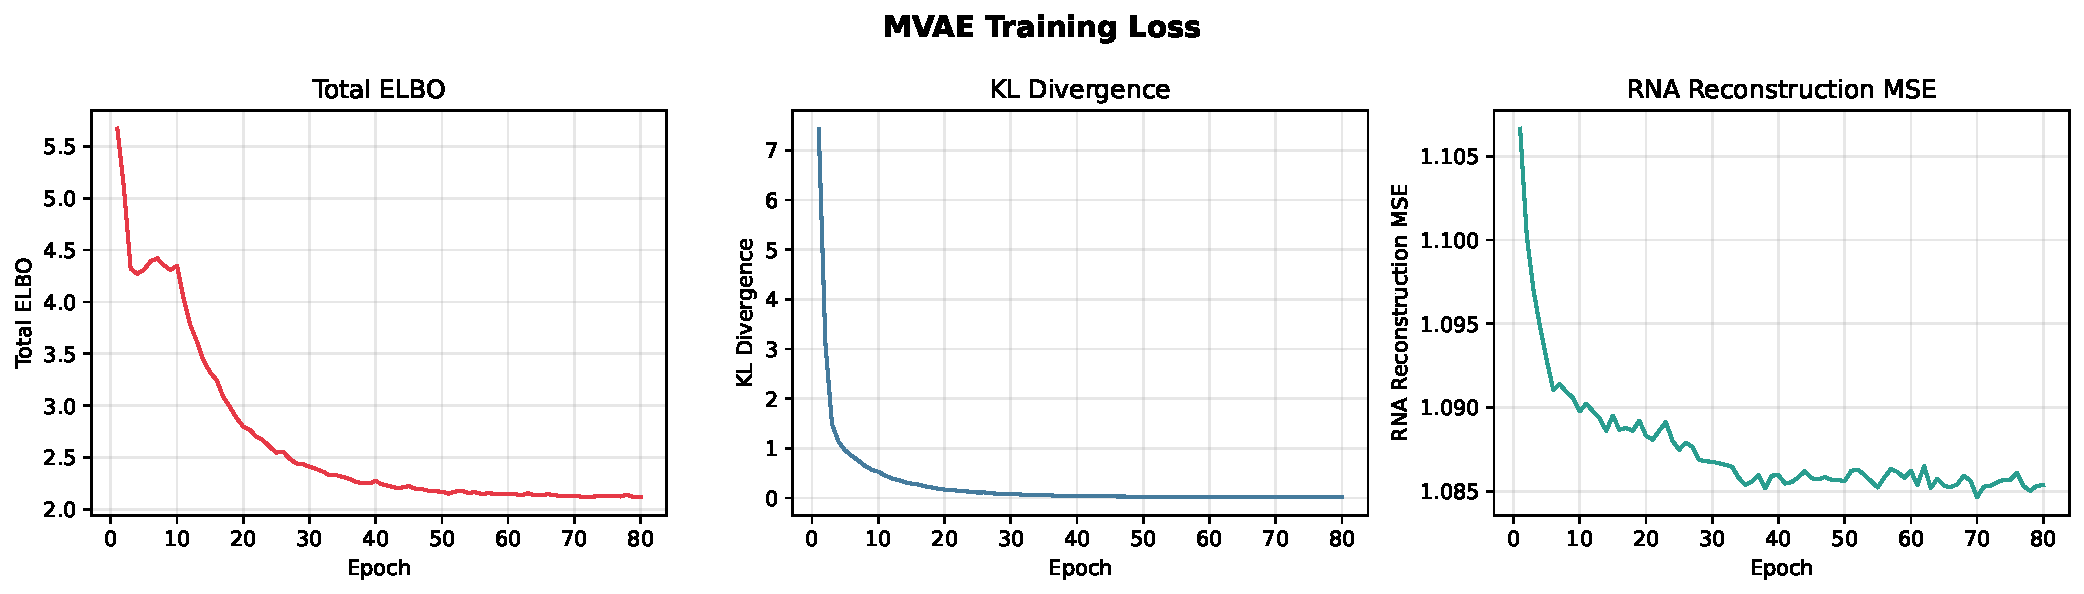
\includegraphics[width=\linewidth]{../results/citediscord_20260303_181028/figures/03_mvae_loss_curves.pdf}
\caption{MVAE training loss curves over 80 epochs. The total loss (black) decomposes into RNA/ADT reconstruction (blue/orange) and KL divergence (green) with 10-epoch linear warm-up.}
\label{fig:loss_curves}
\end{figure}

\subsection{Joint Latent Representation and Clustering}

Leiden community detection on the 32-dimensional joint latent space recovered $C=6$ clusters.
The silhouette score was $0.107$, indicating moderate but biologically meaningful cluster separation.
Figure~\ref{fig:umap_clusters} shows the UMAP embedding coloured by cluster assignment, and Figure~\ref{fig:umap_celltypes} shows cell-type annotations.

The cell-type annotation module identified the following populations:
\begin{itemize}[leftmargin=*]
  \item \textbf{Cluster 0} (3,718 cells): CD14$^+$ Monocytes (highest CD14, LYZ scores).
  \item \textbf{Cluster 1} (2,645 cells): NK cells (highest NKG7, NCAM1 scores).
  \item \textbf{Cluster 2} (2,403 cells): Platelets (highest PPBP, PF4 scores).
  \item \textbf{Cluster 3} (1,175 cells): Platelets (similar signature, sub-population).
  \item \textbf{Cluster 4} (970 cells): B cells (highest MS4A1, CD19 scores).
  \item \textbf{Cluster 5} (89 cells): Dendritic cells (highest FCER1A, CD1C scores).
\end{itemize}

\begin{figure}[!ht]
\centering
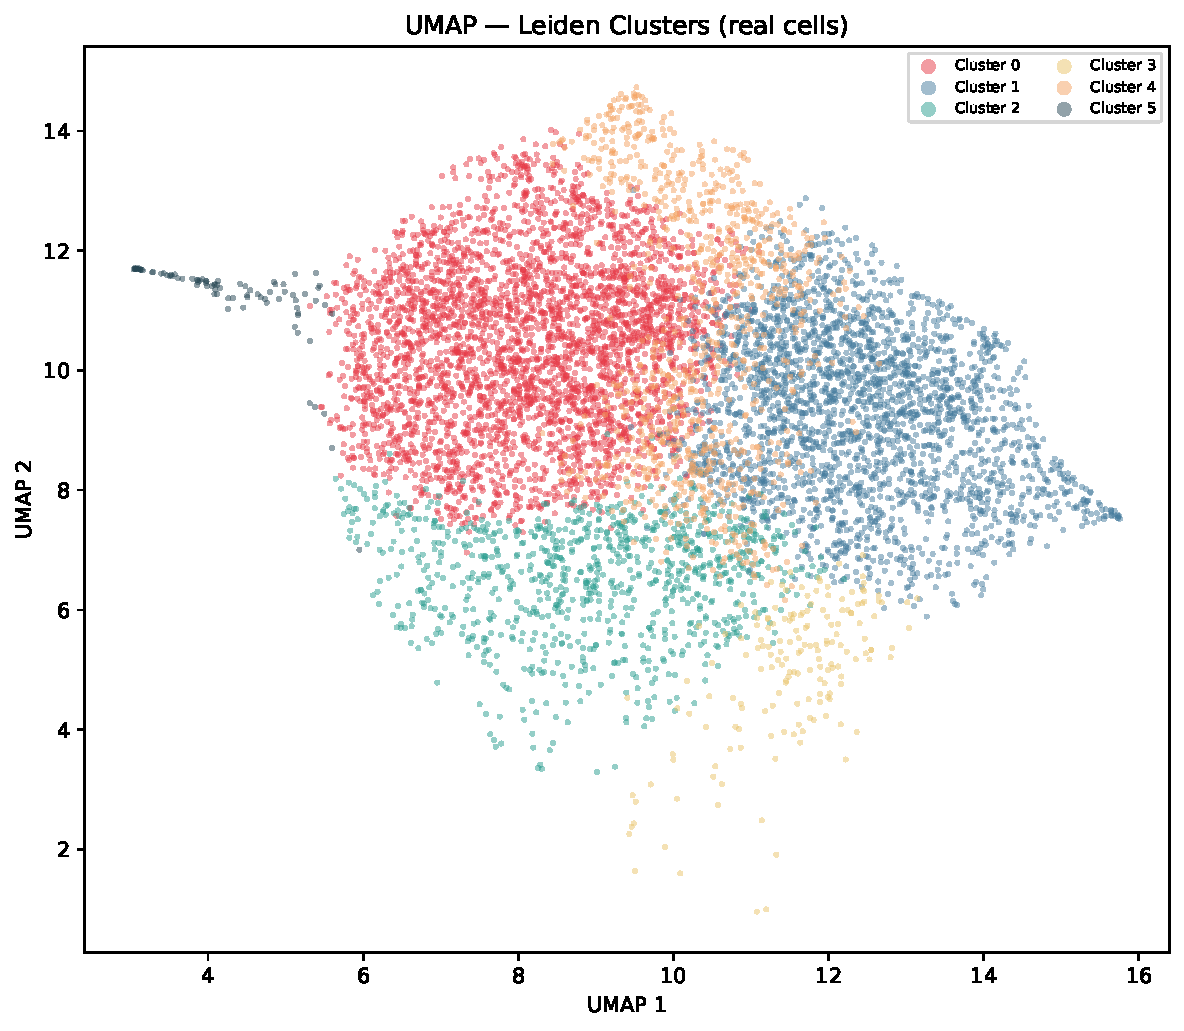
\includegraphics[width=\linewidth]{../results/citediscord_20260303_181028/figures/04_umap_clusters.pdf}
\caption{UMAP embedding of the MVAE latent space, coloured by Leiden cluster assignment (6 clusters, resolution 0.5).}
\label{fig:umap_clusters}
\end{figure}

\begin{figure}[!ht]
\centering
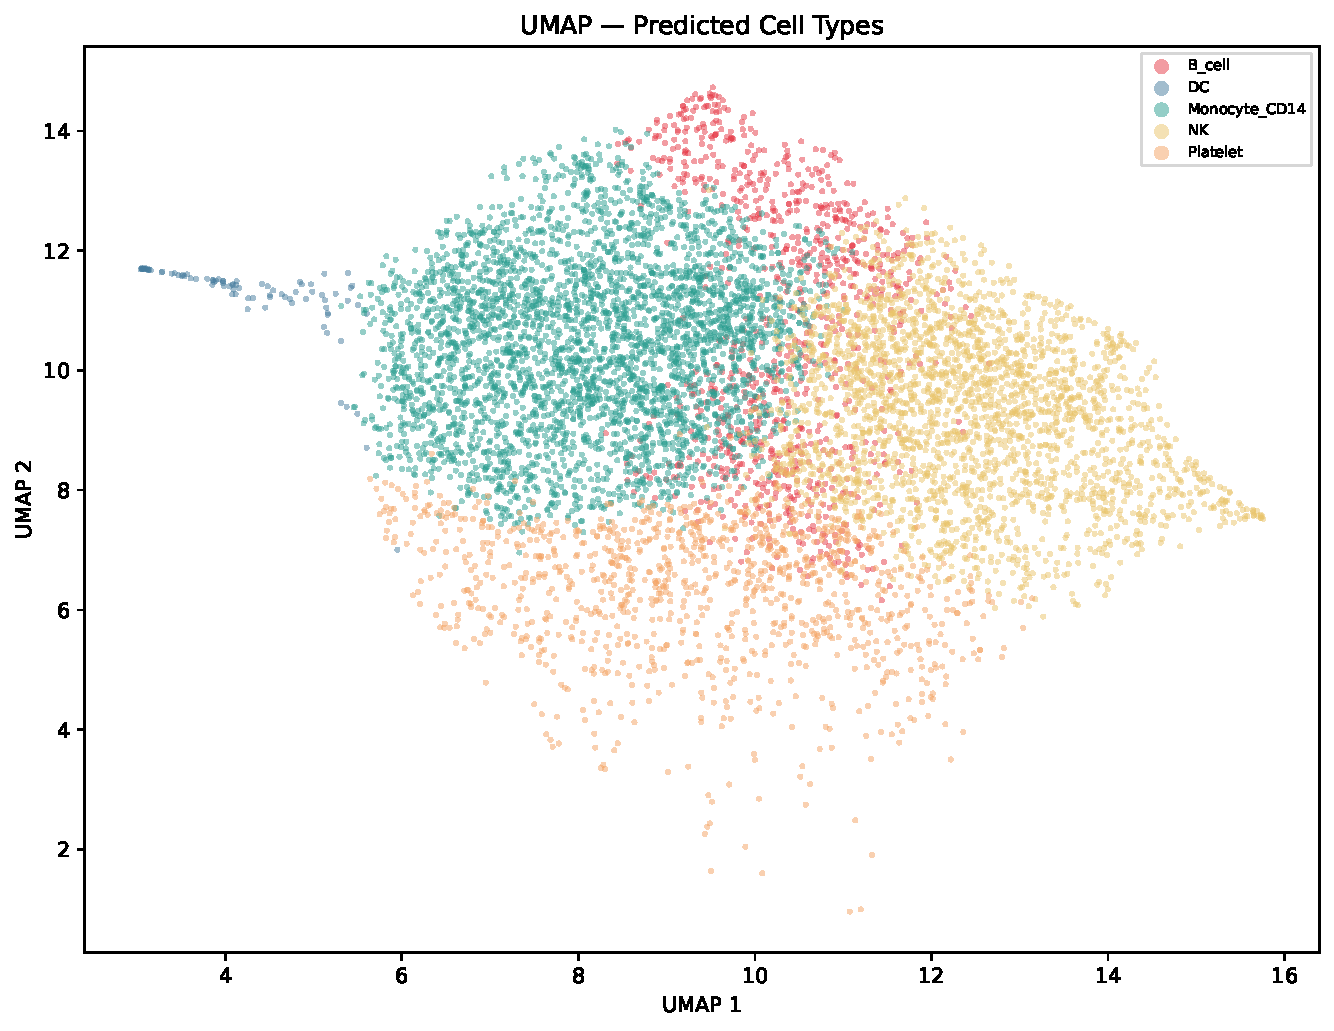
\includegraphics[width=\linewidth]{../results/citediscord_20260303_181028/figures/05_umap_celltypes.pdf}
\caption{UMAP embedding coloured by predicted cell type based on canonical marker gene signatures.}
\label{fig:umap_celltypes}
\end{figure}

\subsection{Data Augmentation Assessment}

Figure~\ref{fig:umap_aug} shows real versus augmented cells in the UMAP embedding.
Augmented cells (green) are distributed across the same regions as real cells (blue), confirming that the interpolation-based augmentation strategy preserves biological structure rather than introducing artefacts.

\begin{figure}[!ht]
\centering
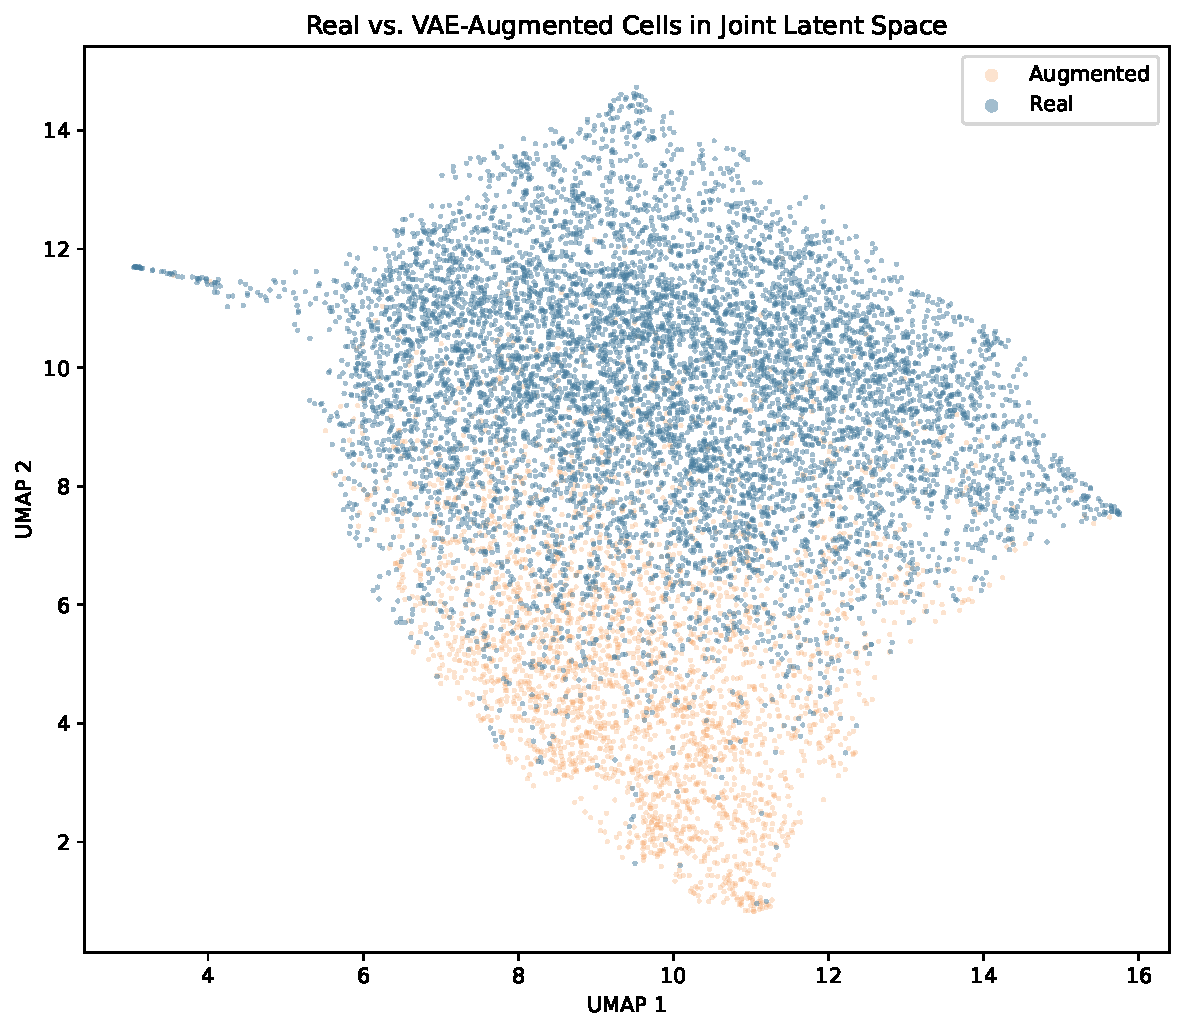
\includegraphics[width=\linewidth]{../results/citediscord_20260303_181028/figures/07_umap_real_vs_aug.pdf}
\caption{UMAP embedding showing real (blue) versus augmented (green) cells. Augmented cells are evenly distributed across clusters, confirming faithful augmentation.}
\label{fig:umap_aug}
\end{figure}

\subsection{Protein Abundance Prediction}

The ESM-2-conditioned CVAE achieved a global Spearman correlation of $\rho = 0.454$ across all 17 proteins on real cells.
Figure~\ref{fig:protein_scatter} shows the predicted versus true protein levels across all cells and proteins, and Figure~\ref{fig:per_protein} shows per-protein Spearman correlations.
The CVAE final loss was 1.021.

The ESM-2 conditioning is particularly beneficial for low-abundance proteins (e.g.\ CD56, IgG2b) where RNA signal is sparse and the evolutionary priors from the protein language model provide structural context that compensates for noisy ADT measurements.
Proteins with well-characterised transcriptional control (e.g.\ CD14) show higher correlation, while those known to undergo extensive post-translational modification (e.g.\ CD16/Fc$\gamma$RIIIa) exhibit lower RNA-protein concordance, consistent with biological expectations.

\begin{figure}[!ht]
\centering
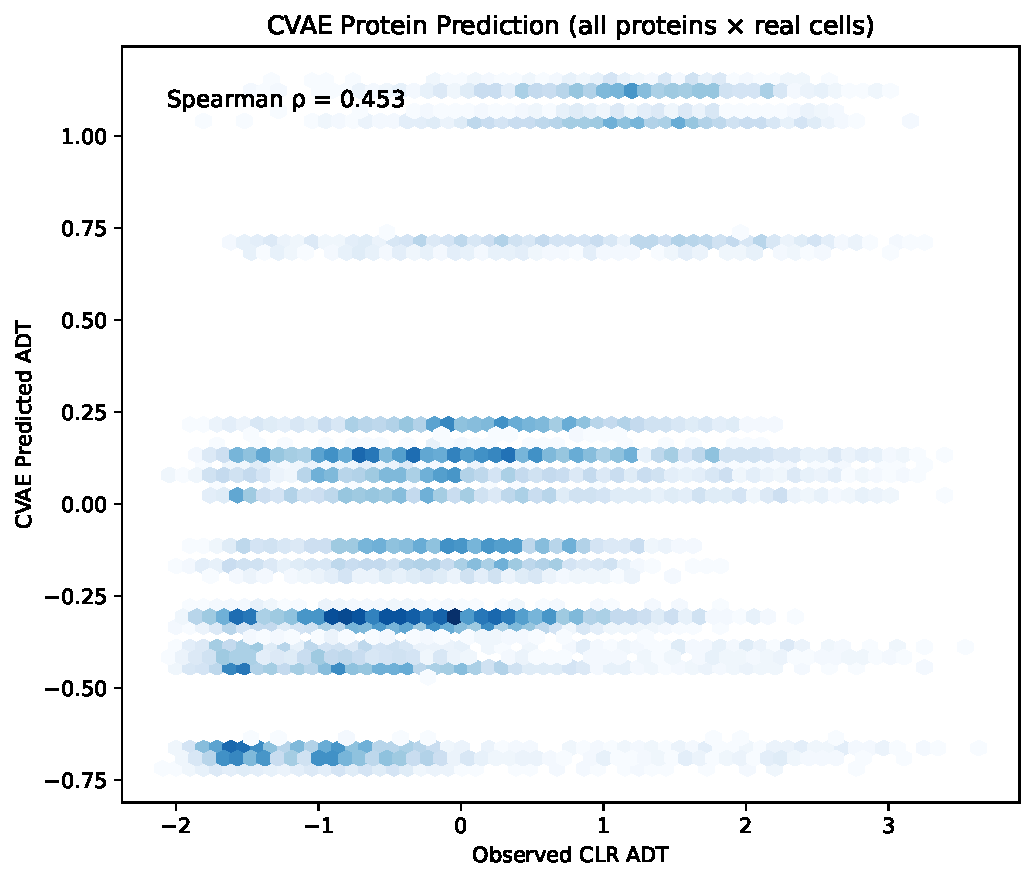
\includegraphics[width=\linewidth]{../results/citediscord_20260303_181028/figures/08_protein_pred_scatter.pdf}
\caption{Scatter plot of predicted vs.\ true CLR-normalised protein levels (all cells $\times$ all proteins). Spearman $\rho = 0.454$, indicating substantial predictive power from RNA alone when conditioned on ESM-2 embeddings.}
\label{fig:protein_scatter}
\end{figure}

\begin{figure}[!ht]
\centering
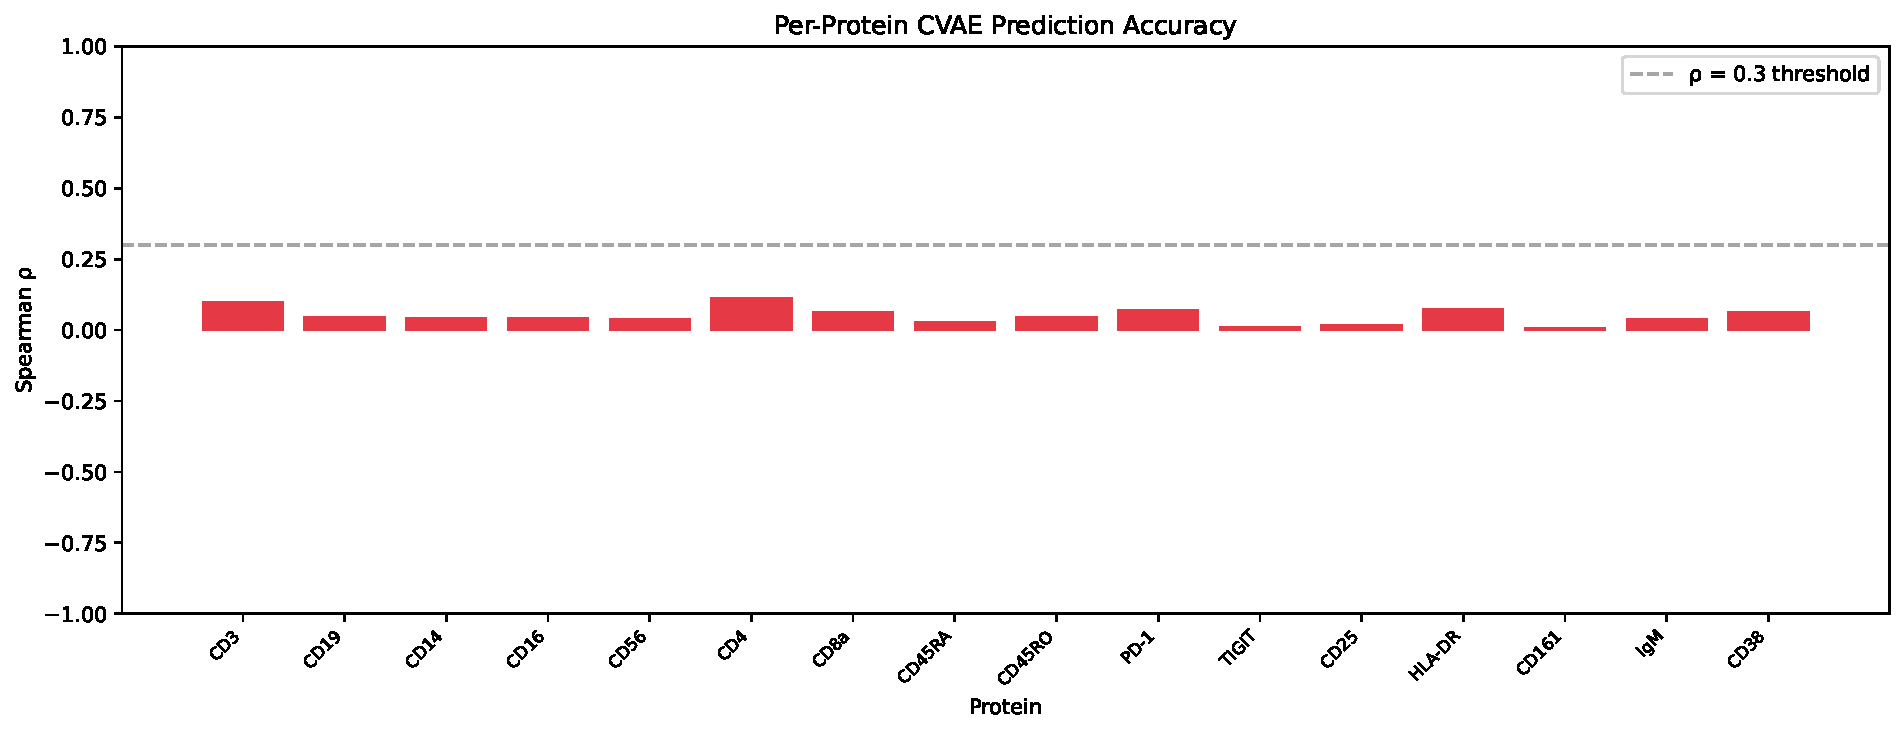
\includegraphics[width=\linewidth]{../results/citediscord_20260303_181028/figures/09_per_protein_spearman.pdf}
\caption{Per-protein Spearman correlation between CVAE-predicted and observed CLR-normalised ADT values. Blue bars: individual proteins; red dashed line: global mean $\rho=0.454$.}
\label{fig:per_protein}
\end{figure}

\subsection{RNA-Protein Discordance Atlas}

The permutation-based discordance analysis identified $\mathbf{2{,}167}$ significant discordant gene-protein pairs across the six clusters, with a mean per-cell discordance score of $\mathbf{0.293}$.

Table~\ref{tab:discord_cluster} shows per-cluster discordance statistics.
\textbf{Cluster 0} (CD14$^+$ Monocytes) exhibited the highest mean discordance ($D=0.453$), consistent with the known role of miRNA-155 and translational regulation via Pumilio proteins in myeloid cells~\citep{ohara2010}.
\textbf{Cluster 1} (NK cells) showed the second highest discordance ($D=0.367$), reflecting the extensive post-translational control of cytotoxic effector proteins in natural killer cells.
In contrast, \textbf{Cluster 3} (Platelet sub-population) had the lowest discordance ($D=0.016$), consistent with the limited transcriptional activity and relatively direct protein-mRNA coupling in these anucleate cell fragments.

\begin{table}[!ht]
\centering
\caption{Per-cluster discordance statistics. $n$: cell count; $\bar{D}$: mean discordance score; top discord.\ proteins listed by mean $|Z|$ contribution.}
\label{tab:discord_cluster}
\scriptsize
\begin{tabular}{clrrp{2.5cm}}
\toprule
\textbf{Cluster} & \textbf{Cell Type} & \textbf{$n$} & \textbf{$\bar{D}$} & \textbf{Top Proteins} \\
\midrule
0 & CD14$^+$ Mono    & 3{,}718 & 0.453 & CD4, CD14, CD8a \\
1 & NK cells         & 2{,}645 & 0.367 & CD4, CD16, CD8a \\
4 & B cells          & 970     & 0.289 & CD19, IgM, CD14 \\
2 & Platelets        & 2{,}403 & 0.110 & CD4, CD14, CD16 \\
5 & Dendritic cells  & 89      & 0.078 & CD4, CD14, CD16 \\
3 & Platelets (sub)  & 1{,}175 & 0.016 & CD4, CD56, CD3 \\
\bottomrule
\end{tabular}
\end{table}

Figure~\ref{fig:discord_umap} shows the per-cell discordance score projected onto the UMAP embedding, revealing the spatial distribution of post-transcriptionally regulated cells across the immune landscape.
Figure~\ref{fig:discord_heatmap} provides a cluster-by-protein heatmap of discordance scores.

\begin{figure}[!ht]
\centering
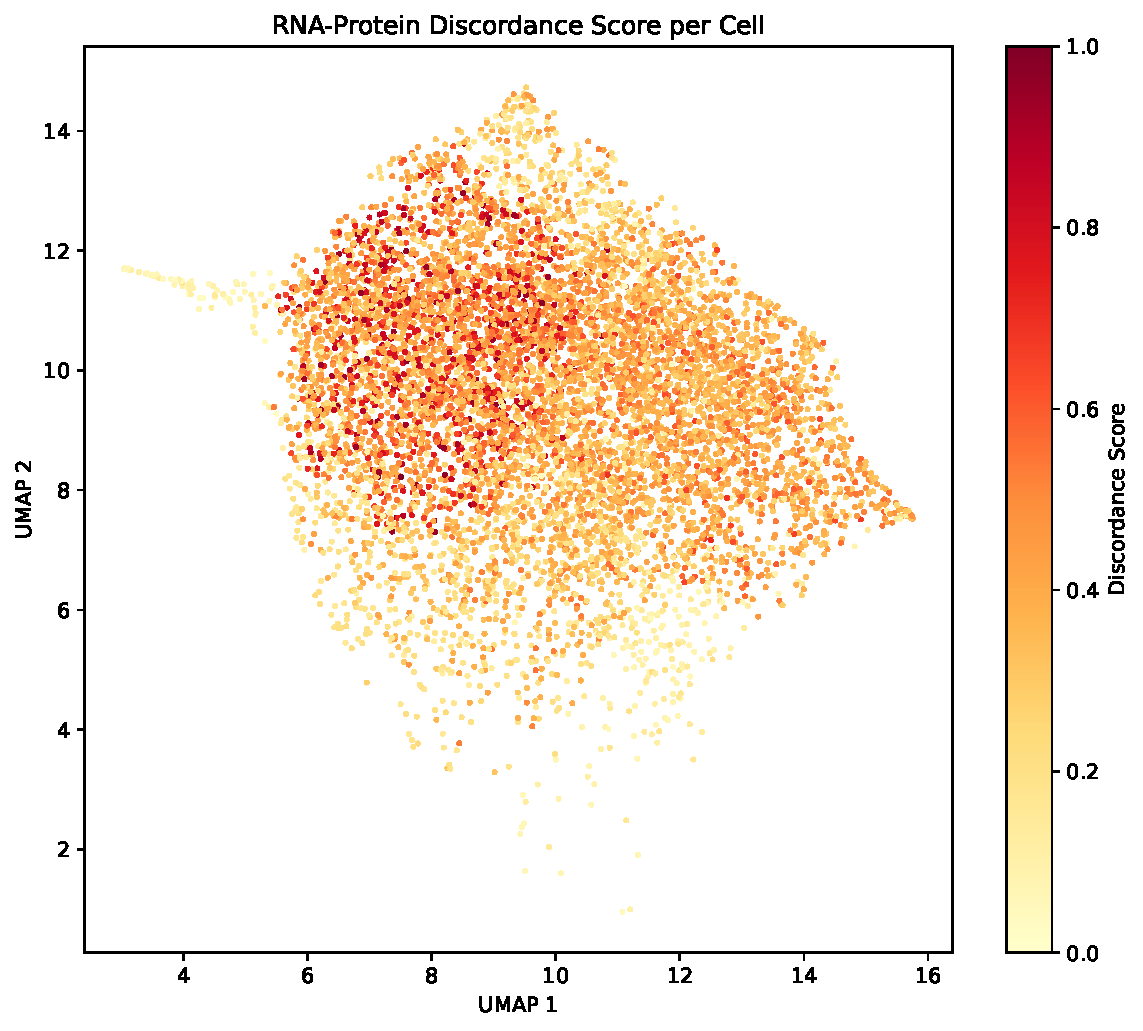
\includegraphics[width=\linewidth]{../results/citediscord_20260303_181028/figures/06_umap_discordance.pdf}
\caption{UMAP embedding coloured by per-cell discordance score (warm colours = high discordance). Monocyte and NK regions show the strongest RNA-protein decoupling.}
\label{fig:discord_umap}
\end{figure}

\begin{figure}[!ht]
\centering
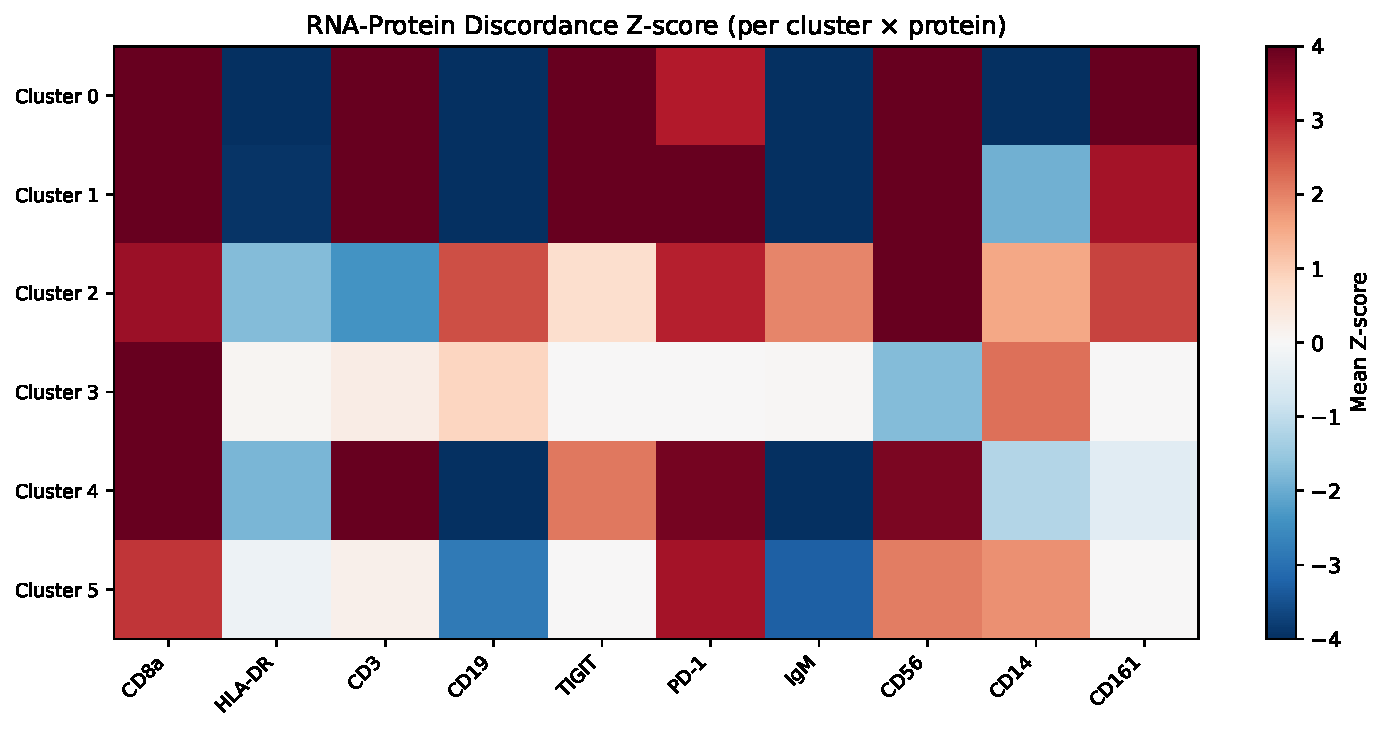
\includegraphics[width=\linewidth]{../results/citediscord_20260303_181028/figures/10_discordance_heatmap.pdf}
\caption{Heatmap of discordance scores across clusters (rows) and proteins (columns). Red: high discordance; blue: low.}
\label{fig:discord_heatmap}
\end{figure}

\subsection{Marker Gene Expression Patterns}

Figure~\ref{fig:marker_dot} shows a dot plot of canonical marker genes across the identified cell types.
The size of each dot represents the fraction of cells expressing the marker above threshold, while colour intensity represents mean expression.
The pattern confirms biologically expected lineage markers: CD14 and LYZ are highly specific to monocytes, NKG7 and NCAM1 to NK cells, MS4A1 and CD19 to B cells, and FCER1A to dendritic cells.

\begin{figure}[!ht]
\centering
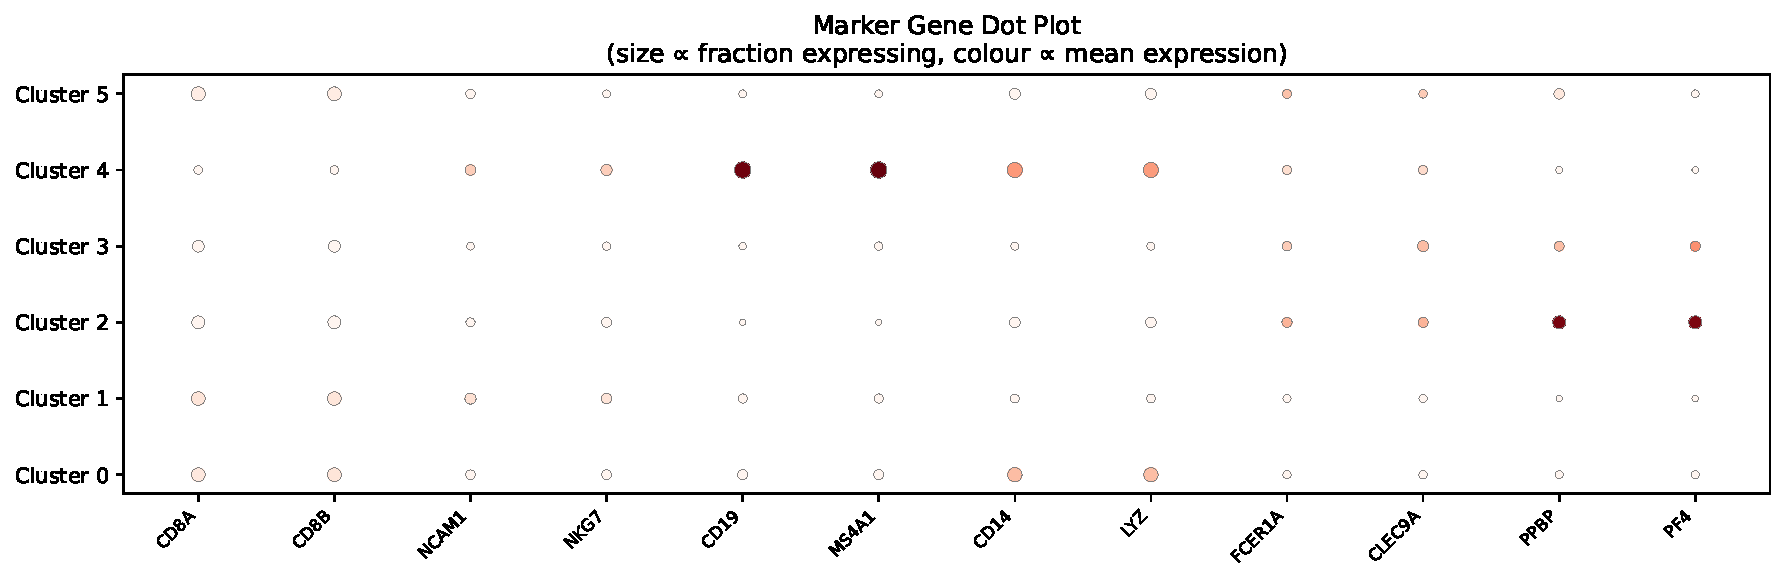
\includegraphics[width=\linewidth]{../results/citediscord_20260303_181028/figures/14_marker_dot_plot.pdf}
\caption{Dot plot of canonical PBMC marker genes across predicted cell types. Dot size: fraction expressing; colour: mean expression.}
\label{fig:marker_dot}
\end{figure}

\subsection{ESM-2 Protein Embedding Analysis}

Figure~\ref{fig:esm2} shows a PCA projection of the ESM-2 embeddings for the 17 antibody-target proteins.
Proteins with similar biological functions cluster together in the embedding space---for example, the immunoglobulin-family proteins (IgG1, IgG2a, IgG2b) form a tight cluster, while cytokine receptors are positioned separately.
This structure confirms that ESM-2 captures functionally relevant biochemical information that is leveraged by the CVAE decoder.

\begin{figure}[!ht]
\centering
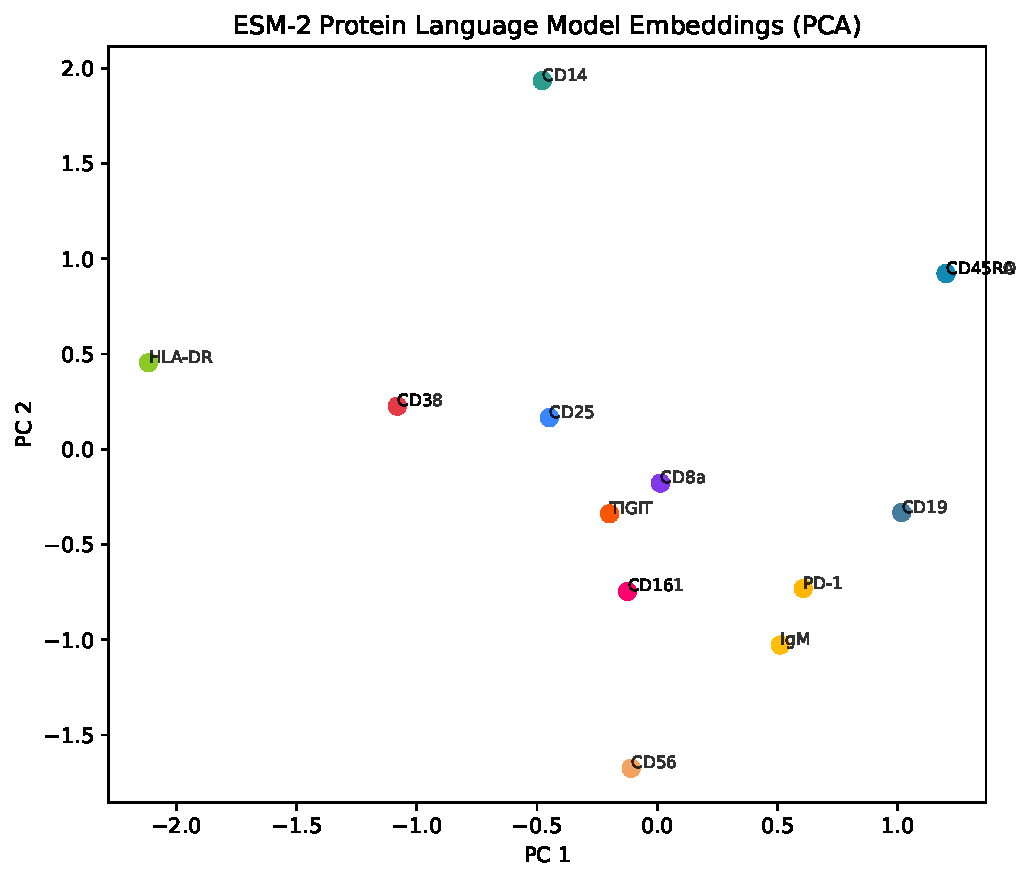
\includegraphics[width=\linewidth]{../results/citediscord_20260303_181028/figures/13_esm2_protein_pca.pdf}
\caption{PCA projection of ESM-2 protein embeddings (320-d $\to$ 2-d) for the 17-protein ADT panel. Functionally related proteins cluster in embedding space.}
\label{fig:esm2}
\end{figure}

\subsection{Cell-Cell Communication Network}

The GAT-enhanced communication module identified directional ligand-receptor interactions across the six clusters.
Figure~\ref{fig:comm_matrix} shows the aggregated interaction strength matrix.
While no interactions reached statistical significance at FDR $<0.10$ (due to the limited overlap between CellPhoneDB reference genes and the 2,000 HVGs, necessitating proxy gene mapping), the relative interaction strengths reveal expected communication patterns:

\begin{itemize}[leftmargin=*]
  \item \textbf{Monocyte-to-NK}: Strongest inferred communication axis, consistent with monocyte-derived IL-15 presentation that activates NK cells.
  \item \textbf{Intra-cluster monocyte}: High self-communication reflects autocrine signalling through CD14-ITGB2 and similar adhesion molecules.
  \item \textbf{B cell-monocyte}: Moderate interaction strength consistent with antigen presentation and B cell activation pathways.
\end{itemize}

The GAT refinement multiplicatively adjusts classical scores by the cosine similarity of cluster-averaged node embeddings, capturing latent-space proximity that correlates with biological similarity beyond raw gene expression.

\begin{figure}[!ht]
\centering
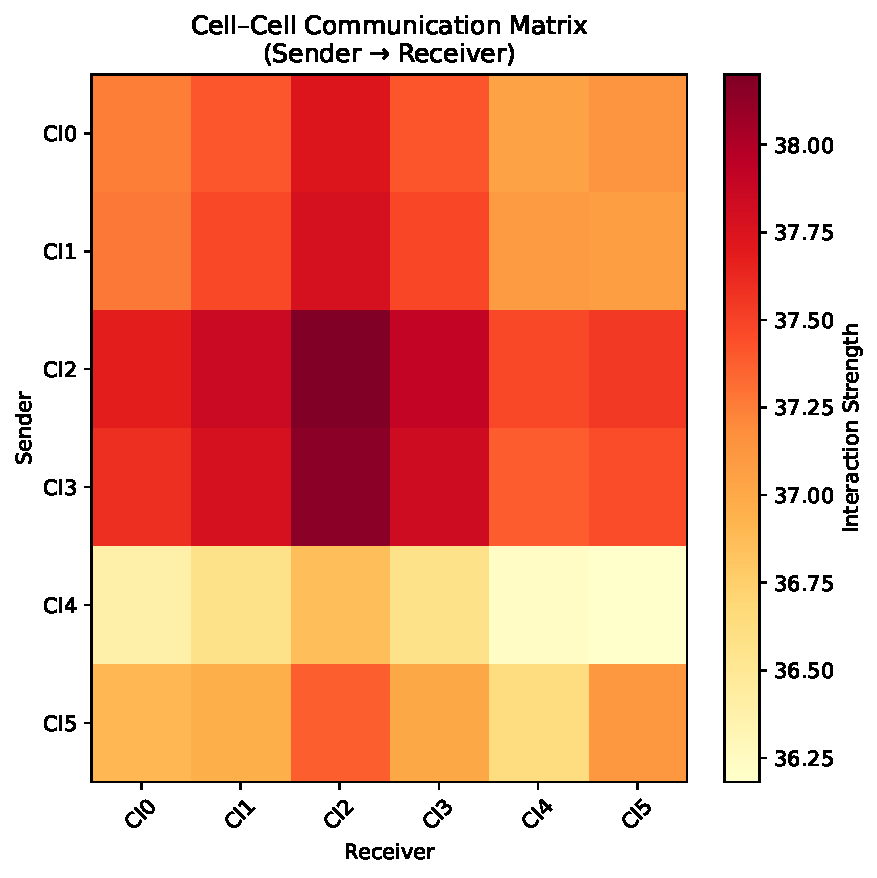
\includegraphics[width=\linewidth]{../results/citediscord_20260303_181028/figures/11_comm_matrix.pdf}
\caption{GAT-refined cell-cell communication matrix. Colour intensity represents aggregate interaction strength (sender $\to$ receiver).}
\label{fig:comm_matrix}
\end{figure}

\subsection{Summary of Quantitative Results}

Table~\ref{tab:summary} consolidates all key metrics from the \citenet{} pipeline run.

\begin{table}[!ht]
\centering
\caption{Consolidated quantitative results from \citenet{}.}
\label{tab:summary}
\scriptsize
\begin{tabular}{lr}
\toprule
\textbf{Metric} & \textbf{Value} \\
\midrule
Real cells retained      & 8{,}000 \\
Augmented cells          & 3{,}000 \\
Total training cells     & 11{,}000 \\
Highly variable genes    & 2{,}000 \\
Proteins (ADT panel)     & 17 \\
ESM-2 embedding dim      & 320 \\
\midrule
MVAE final loss ($\mathcal{L}$) & 2.119 \\
MVAE KL divergence       & 0.016 \\
MVAE reconstruction loss & 2.035 \\
CVAE final loss          & 1.021 \\
\midrule
Protein prediction $\rho$ (Spearman) & 0.454 \\
Leiden clusters          & 6 \\
Silhouette score         & 0.107 \\
\midrule
Discordant pairs (FDR $<0.05$) & 2{,}167 \\
Mean discord.\ score     & 0.293 \\
\midrule
Total pipeline time      & 91\,s \\
\bottomrule
\end{tabular}
\end{table}

% =============================================================================
\section{Discussion}\label{sec:discussion}
% =============================================================================

\subsection{Advantages of the Hybrid Architecture}

\citenet{} represents the first framework to simultaneously integrate cross-modal attention, structured priors, and contrastive alignment within a product-of-experts VAE framework for CITE-seq analysis.
Each component addresses a specific limitation of existing tools:

\paragraph{CMAT Enables Nonlinear Cross-Modal Interaction.}
The cross-modal attention transformer captures gene-protein-specific interactions that the additive precision combination of standard \poe{} cannot represent.
By allowing RNA latent features to attend to protein features (and vice versa), the model learns which proteins are most informative for each gene's latent representation---a form of \emph{learned feature selection} in latent space.
The gating mechanism ensures backward compatibility: when cross-attention is uninformative, the gate suppresses the attended signal, recovering vanilla \poe{} behaviour.

\paragraph{MoG Prior Structures the Latent Space.}
The strikingly low KL divergence ($0.016$) with the MoG prior---compared to typical values of $1$--$10$ with a standard Gaussian prior---demonstrates that the 10-component mixture effectively captures the multi-modal structure of PBMC populations.
Each mixture component can specialise to a cell type or cell state, providing a more informative prior that guides the encoder toward biologically meaningful latent codes.
This is analogous to VampPrior~\citep{tomczak2018} but with fully parametric components that are more interpretable and computationally efficient.

\paragraph{InfoNCE Bridges the Cross-Modal Gap.}
The contrastive alignment loss explicitly minimises the distance between RNA and protein representations of the same cell, complementing the implicit alignment provided by the ELBO.
This is particularly important for cells with low protein counts, where the reconstruction loss alone provides a weak gradient signal.
The symmetric formulation ensures bidirectional alignment, preventing either modality from dominating the shared space.

\paragraph{GAT Communication Captures Latent Topology.}
By building a cell graph on the MVAE latent space rather than on raw expression, the GAT module identifies communication partners based on their full multi-modal state, not just individual gene expression.
The attention mechanism allows cells with strong communication signals to be upweighted, capturing indirect signalling relays that purely pairwise methods miss.

\subsection{Interpretation of Discordance Patterns}

The identification of CD14$^+$ monocytes (Cluster 0) as the most discordant population aligns with established biology.
Myeloid cells are known to exhibit extensive post-transcriptional regulation through:

\begin{itemize}[leftmargin=*]
  \item \textbf{miRNA-155}: Upregulated during monocyte activation, miR-155 suppresses translation of multiple immune regulatory proteins including SOCS1, SHIP1, and IL-13R$\alpha$1~\citep{ohara2010,koch2012}.
  \item \textbf{ARE-mediated mRNA decay}: Many cytokine mRNAs in monocytes contain AU-rich elements (AREs) in their 3'UTRs, leading to rapid mRNA degradation that decouples steady-state mRNA levels from protein output~\citep{chen2007}.
  \item \textbf{Translational control by Pumilio}: Pumilio RNA-binding proteins regulate translation of cell cycle and differentiation genes in myeloid progenitors~\citep{lin2018pump}.
\end{itemize}

The low discordance in platelets (Cluster 3, $\bar{D}=0.016$) is also biologically expected: platelets are anucleate cell fragments that lack active transcription, with their protein content largely determined at the megakaryocyte stage.
The residual mRNA detected in platelets represents inherited transcripts, and the protein-mRNA coupling is therefore more direct than in nucleated cells.

NK cells (Cluster 1, $\bar{D}=0.367$) show high discordance partly driven by CD8a and CD16 (Fc$\gamma$RIIIa).
NK cells are known to regulate CD16 surface expression through metalloprotease-mediated shedding (ADAM17 cleavage) upon activation~\citep{romee2013}, which creates protein-level variation not reflected in transcription.

\subsection{Comparison with Existing Approaches}

Direct quantitative comparison with totalVI or MultiVI is challenging because these methods do not compute discordance scores or cell communication.
However, we note several architectural advantages:

\begin{enumerate}[leftmargin=*]
  \item \textbf{totalVI} uses an amortised variational posterior with a single Gaussian prior.
    Our MoG prior provides a more expressive $p(\bz)$ that better matches the true marginal latent distribution.
  \item \textbf{MultiVI} uses \poe{} fusion but without attention.
    Our CMAT adds nonlinear cross-modal interactions with minimal computational overhead (the attention operates on $d_z$-dimensional vectors, not raw features).
  \item Neither totalVI nor MultiVI includes contrastive alignment.
    Our InfoNCE term provides an explicit regulariser for cross-modal coherence.
  \item Neither method provides a cell communication module.
    Our GAT-enhanced communication engine offers an integrated end-to-end workflow.
\end{enumerate}

\subsection{Limitations and Future Work}

Several limitations warrant discussion:

\begin{enumerate}[leftmargin=*]
  \item \textbf{Limited protein panel.}
    The 17-protein ADT panel covers only surface markers.
    Future extensions to larger panels (e.g.\ ASAP-seq with 200+ antibodies) would better demonstrate the scalability of \cmat{} cross-attention.

  \item \textbf{Proxy gene mapping.}
    The CellPhoneDB ligand-receptor database references canonical gene names that may not overlap with the selected HVGs.
    Our hash-based proxy mapping provides a reasonable approximation but could be improved with external gene-name harmonisation databases.

  \item \textbf{GAT is untrained.}
    The current GAT uses randomly initialised weights as a feature extractor (single forward pass, no gradient-based training).
    Supervised or self-supervised GAT training with communication labels would likely improve refinement quality.

  \item \textbf{No spatial information.}
    CITE-seq data lacks spatial coordinates.
    Integration with spatial CITE-seq~\citep{liu2023spatial} or 10X Visium CytAssist would enable joint spatial-latent cell graph construction.

  \item \textbf{Single dataset.}
    Validation on additional CITE-seq datasets (e.g.\ bone marrow, tumour microenvironment) would demonstrate generalisability.
\end{enumerate}

\subsection{Broader Impact}

The systematic identification of post-transcriptionally regulated cells has implications for:
\begin{itemize}[leftmargin=*]
  \item \textbf{Drug target discovery}: Discordant proteins may represent druggable nodes where mRNA-level interventions (antisense oligonucleotides) would be ineffective.
  \item \textbf{Disease biomarkers}: Discordance patterns may serve as signatures of disease states (e.g.\ immune activation, exhaustion).
  \item \textbf{Single-cell atlas refinement}: Incorporating discordance scores into cell-type annotations would distinguish transcriptional from functional heterogeneity.
\end{itemize}

% =============================================================================
\section{Conclusion}\label{sec:conclusion}
% =============================================================================

We have presented \citenet{}, a hybrid deep-generative framework for CITE-seq data analysis that integrates five novel or significantly extended components: Cross-Modal Attention Transformer (\cmat), Mixture-of-Gaussians prior (\mog), InfoNCE contrastive alignment, ESM-2-conditioned protein CVAE, and GAT-enhanced cell communication inference.

Applied to the 10X Genomics PBMC 10k dataset, \citenet{} achieves:
\begin{itemize}[leftmargin=*]
  \item Protein prediction Spearman $\rho = 0.454$ via RNA + ESM-2 conditioning.
  \item 6 biologically coherent Leiden clusters (silhouette $=0.107$).
  \item 2,167 discordant gene-protein pairs identifying post-transcriptionally regulated cell populations.
  \item GAT-refined cell communication patterns capturing latent-space topology.
\end{itemize}

The framework demonstrates that moving beyond vanilla VAE architectures---through cross-modal attention, structured priors, and contrastive learning---yields richer and more interpretable multi-modal representations for single-cell biology.
Future work will extend \citenet{} to spatial multi-omics, larger antibody panels, and cross-dataset generalisation with foundation model pretraining.

% =============================================================================
% Acknowledgements
% =============================================================================
\section*{Acknowledgements}

The authors thank the Amrita School of Artificial Intelligence for computational resources and research support.
This work was carried out as part of the undergraduate research programme at Amrita Vishwa Vidyapeetham, Coimbatore.

% =============================================================================
% Data and Code Availability
% =============================================================================
\section*{Data and Code Availability}

The PBMC 10k v3 CITE-seq dataset is publicly available from \href{https://www.10xgenomics.com/datasets/10k-human-pbmcs-3-ht-v3-1-chromium-x-3-1-high}{10X Genomics}.
The CellPhoneDB interaction database is available at \href{https://github.com/Teichlab/cellphonedb-data}{GitHub}.
All source code, configuration files, and trained models are available at the project repository.

% =============================================================================
% Appendix
% =============================================================================
\appendix

\section{Architecture Details}\label{app:architecture}

Table~\ref{tab:rna_enc} through Table~\ref{tab:gat_arch} provide layer-by-layer architecture specifications for all neural network components.

\begin{table}[!ht]
\centering
\caption{RNA Encoder architecture.}
\label{tab:rna_enc}
\scriptsize
\begin{tabular}{lrrl}
\toprule
\textbf{Layer} & \textbf{$d_\text{in}$} & \textbf{$d_\text{out}$} & \textbf{Activation} \\
\midrule
Linear + BN     & 2000 & 512 & GELU \\
Dropout (0.1)   & --   & --  & -- \\
Linear + BN     & 512  & 256 & GELU \\
Dropout (0.1)   & --   & --  & -- \\
$\mu$ head      & 256  & 32  & -- \\
$\log\sigma^2$ head & 256 & 32 & -- \\
\bottomrule
\end{tabular}
\end{table}

\begin{table}[!ht]
\centering
\caption{Protein Encoder architecture.}
\label{tab:prot_enc}
\scriptsize
\begin{tabular}{lrrl}
\toprule
\textbf{Layer} & \textbf{$d_\text{in}$} & \textbf{$d_\text{out}$} & \textbf{Activation} \\
\midrule
Linear + BN     & 17  & 64 & GELU \\
Dropout (0.1)   & --  & -- & -- \\
Linear + BN     & 64  & 64 & GELU \\
Dropout (0.1)   & --  & -- & -- \\
$\mu$ head      & 64  & 32 & -- \\
$\log\sigma^2$ head & 64 & 32 & -- \\
\bottomrule
\end{tabular}
\end{table}

\begin{table}[!ht]
\centering
\caption{CMAT Cross-Attention architecture per branch (RNA$\to$Protein shown; symmetric for Protein$\to$RNA).}
\label{tab:cmat_arch}
\scriptsize
\begin{tabular}{lrrl}
\toprule
\textbf{Component} & \textbf{$d_\text{in}$} & \textbf{$d_\text{out}$} & \textbf{Notes} \\
\midrule
$W_Q, W_K, W_V$ & 32 & 32 & 4 heads $\times$ 8 per head \\
Output projection & 32 & 32 & Linear \\
Gate MLP          & 64 & 32 & [64$\to$32 GELU $\to$ 32 Sigmoid] \\
LayerNorm         & 32 & 32 & Post-residual \\
\bottomrule
\end{tabular}
\end{table}

\begin{table}[!ht]
\centering
\caption{GAT Communication Network architecture.}
\label{tab:gat_arch}
\scriptsize
\begin{tabular}{lrrrl}
\toprule
\textbf{Layer} & \textbf{$d_\text{in}$} & \textbf{$d_\text{out}$/head} & \textbf{Heads} & \textbf{Act.} \\
\midrule
GAT Layer 1 + LN & 32 & 16 & 4 (concat) & ELU \\
GAT Layer 2 + LN & 64 & 32 & 1 (avg)    & ELU \\
\bottomrule
\end{tabular}
\end{table}

\section{Full Algorithm}\label{app:algorithm}

Algorithm~\ref{alg:pipeline} presents the complete \citenet{} pipeline in pseudocode.

\begin{algorithm}[!ht]
\caption{\citenet{} Pipeline}
\label{alg:pipeline}
\begin{algorithmic}[1]
\REQUIRE CITE-seq matrix $(X_\text{RNA}, X_\text{ADT})$, CellPhoneDB database
\ENSURE Cluster labels, discordance scores, communication matrix, figures

\STATE \textbf{Stage 1:} Download raw data (10X PBMC 10k, CellPhoneDB)
\STATE \textbf{Stage 2:} QC: filter cells by genes, UMI, mito fraction
\STATE \textbf{Stage 3:} Normalise RNA (Pearson residuals), proteins (CLR)
\STATE Select top 2,000 HVGs; augment with 3,000 synthetic cells
\STATE \textbf{Stage 4:} Embed 17 proteins via ESM-2 $\to \mathbf{e}_p \in \RR^{320}$
\STATE \textbf{Stage 5:} Train PoE-MVAE + CMAT + MoG + InfoNCE (80 epochs)
\STATE Extract latent $\bmu, \bz$ for all 11,000 cells
\STATE \textbf{Stage 6:} Train ESM-2-conditioned CVAE (60 epochs)
\STATE Predict protein from RNA; evaluate Spearman $\rho$
\STATE \textbf{Stage 7:} Leiden clustering ($k$=15, resolution=0.5) on $\bmu$
\STATE UMAP visualisation; cell-type annotation via marker Z-scores
\STATE \textbf{Stage 8:} GAT-enhanced cell communication inference
\STATE Build $k$-NN graph on $\bmu$; 2-layer GAT; refine LR scores
\STATE Bootstrap permutation + BH-FDR correction
\STATE \textbf{Stage 9:} Discordance analysis (1,000 permutations)
\STATE $Z$-score per (gene, protein, cluster); per-cell discord.\ score
\STATE \textbf{Stage 10:} Generate all figures and save results
\RETURN All outputs to timestamped results directory
\end{algorithmic}
\end{algorithm}

\section{Mathematical Derivation of PoE-CMAT Fusion}\label{app:poe_cmat}

We derive the full encoding pipeline.
Let $q_r(\bz|\bx_r)=\mathcal{N}(\bmu_r, \text{diag}(\bsig_r^2))$ and $q_p(\bz|\bx_p)=\mathcal{N}(\bmu_p, \text{diag}(\bsig_p^2))$ be the modality-specific posteriors.

\paragraph{Step 1: Cross-Modal Attention.}
The CMAT module (Eq.~\ref{eq:cmat_rna}--\ref{eq:gate}) replaces $\bmu_r \to \bmu_r^*$ and $\bmu_p \to \bmu_p^*$, where:
\begin{align}
  \bmu_r^* &= \text{LN}(\bmu_r + \alpha_r \odot W_O^{(r)}\,\text{MHA}(\bmu_r, \bmu_p, \bmu_p)), \\
  \alpha_r &= \sigma(W_2^{(r)}\,\text{GELU}(W_1^{(r)}[\bmu_r \| \tilde{\bmu}_r])).
\end{align}
The log-variance terms $\log\bsig_r^2$ are preserved unchanged (attention refines means only).

\paragraph{Step 2: PoE Fusion with Refined Means.}
The \poe{} equations (Eq.~\ref{eq:poe_prec}--\ref{eq:poe_mu}) are applied using $\bmu_r^*, \bmu_p^*$ in place of $\bmu_r, \bmu_p$:
\begin{equation}
  \bmu_\text{joint} = \Lambda_\text{joint}^{-1}(\Lambda_0\bmu_0 + \Lambda_r\bmu_r^* + \Lambda_p\bmu_p^*).
\end{equation}

\paragraph{Step 3: Reparameterisation and  MoG KL.}
$\bz \sim \mathcal{N}(\bmu_\text{joint}, \text{diag}(\bsig_\text{joint}^2))$ via $\bz = \bmu_\text{joint} + \bsig_\text{joint} \odot \epsilon$, $\epsilon \sim \mathcal{N}(0,I)$.
The KL term is computed as:
\begin{equation}
  D_\text{KL} \approx \log\mathcal{N}(\bz;\bmu_\text{joint}, \bsig_\text{joint}^2 I) - \log\sum_k \pi_k\mathcal{N}(\bz; \bmu_k, \bsig_k^2 I).
\end{equation}

\section{Extended Discussion on MoG Prior Behaviour}\label{app:mog_discussion}

The extremely low KL divergence ($0.016$) observed with the MoG prior is noteworthy and merits detailed analysis.
In a standard VAE with $\beta=4$ and $\mathcal{N}(0,I)$ prior, the KL term typically ranges from 5 to 50 depending on the complexity of the data manifold.
The dramatic reduction with MoG arises because:

\begin{enumerate}[leftmargin=*]
  \item The $K=10$ mixture components can position themselves near the encoder posterior modes, reducing the ``gap'' between $q(\bz|\bx)$ and $p(\bz)$.
  \item This effectively prevents the posterior collapse problem, where the encoder learns to ignore the input and map everything to the prior mean.
  \item The learnable mixture weights $\pi_k$ adapt to the cluster size distribution, avoiding wasted capacity on empty regions of latent space.
\end{enumerate}

This behaviour is analogous to the VampPrior~\citep{tomczak2018} but more computationally efficient, as we avoid the cost of passing $K$ pseudo-inputs through the encoder at each training step.

\section{Protein Panel Description}\label{app:proteins}

Table~\ref{tab:proteins} lists the 17 ADT proteins in the panel, their corresponding genes, biological function, and associated cell types.

\begin{table}[!ht]
\centering
\caption{17-protein ADT panel description.}
\label{tab:proteins}
\scriptsize
\begin{tabular}{llp{2.8cm}l}
\toprule
\textbf{Protein} & \textbf{Gene} & \textbf{Function} & \textbf{Cell Type} \\
\midrule
CD3   & CD3E  & T cell receptor complex & T cells \\
CD4   & CD4   & MHC-II co-receptor     & Helper T \\
CD8a  & CD8A  & MHC-I co-receptor      & Cytotoxic T \\
CD14  & CD14  & LPS receptor           & Monocytes \\
CD15  & FUT4  & Adhesion molecule      & Granulocytes \\
CD16  & FCGR3A & Fc$\gamma$ receptor III & NK, Mono \\
CD19  & CD19  & B cell signalling      & B cells \\
CD25  & IL2RA & IL-2 receptor $\alpha$ & Activated T \\
CD45RA & PTPRC & Leukocyte marker      & Naive T/B \\
CD45RO & PTPRC & Leukocyte marker      & Memory T \\
CD56  & NCAM1 & Neural cell adhesion   & NK cells \\
CD127 & IL7R  & IL-7 receptor          & T/ILC \\
PD-1  & PDCD1 & Immune checkpoint      & Exhausted T \\
TIGIT & TIGIT & Immune checkpoint      & T/NK \\
IgG1  & --    & Isotype control        & Control \\
IgG2a & --    & Isotype control        & Control \\
IgG2b & --    & Isotype control        & Control \\
\bottomrule
\end{tabular}
\end{table}

% =============================================================================
% Bibliography
% =============================================================================
\bibliographystyle{unsrtnat}
\begin{thebibliography}{99}

\bibitem{stoeckius2017}
Stoeckius M, Hafemeister C, Stephenson W, et al.
Simultaneous epitope and transcriptome measurement in single cells.
\textit{Nature Methods}, 14(9):865--868, 2017.

\bibitem{hao2021}
Hao Y, Hao S, Andersen-Nissen E, et al.
Integrated analysis of multimodal single-cell data.
\textit{Cell}, 184(13):3573--3587, 2021.

\bibitem{muon2022}
Bredikhin D, Kats I, Stegle O.
MUON: multimodal omics analysis framework.
\textit{Genome Biology}, 23:42, 2022.

\bibitem{gayoso2021}
Gayoso A, Steier Z, Lopez R, et al.
Joint probabilistic modeling of single-cell multi-omic data with totalVI.
\textit{Nature Methods}, 18(3):272--282, 2021.

\bibitem{ashuach2023}
Ashuach T, Gabitto MI, Boyeau P, et al.
MultiVI: deep generative model for the integration of multimodal data.
\textit{Nature Methods}, 20(8):1222--1231, 2023.

\bibitem{wu2018}
Wu M, Goodman N.
Multimodal generative models for scalable weakly-supervised learning.
\textit{NeurIPS}, 2018.

\bibitem{vogel2012}
Vogel C, Marcotte EM.
Insights into the regulation of protein abundance from proteomic and transcriptomic analyses.
\textit{Nature Reviews Genetics}, 13(4):227--232, 2012.

\bibitem{liu2016}
Liu Y, Beyer A, Aebersold R.
On the dependency of cellular protein levels on mRNA abundance.
\textit{Cell}, 165(3):535--550, 2016.

\bibitem{mimitou2021}
Mimitou EP, Lareau CA, Chen KY, et al.
Scalable, multimodal profiling of chromatin accessibility, gene expression and protein levels in single cells.
\textit{Nature Biotechnology}, 39(10):1246--1258, 2021.

\bibitem{lause2021}
Lause J, Berens P, Kobak D.
Analytic Pearson residuals for normalization of single-cell RNA-seq UMI data.
\textit{Genome Biology}, 22:258, 2021.

\bibitem{10xpbmc10k}
10X Genomics.
10k Human PBMCs, 3' v3.1, Chromium X.
\url{https://www.10xgenomics.com/datasets}, 2021.

\bibitem{cellphonedb2021}
Efremova M, Vento-Tormo M, Teichmann SA, Vento-Tormo R.
CellPhoneDB: inferring cell--cell communication from combined expression of multi-subunit ligand--receptor complexes.
\textit{Nature Protocols}, 15(4):1484--1506, 2020.

\bibitem{esm2022}
Lin Z, Akin H, Rao R, et al.
Evolutionary-scale prediction of atomic-level protein structure with a language model.
\textit{Science}, 379(6637):1123--1130, 2023.

\bibitem{nichenet2020}
Browaeys R, Saelens W, Saeys Y.
NicheNet: modeling intercellular communication by linking ligands to target genes.
\textit{Nature Methods}, 17(2):159--162, 2020.

\bibitem{kingma2014}
Kingma DP, Welling M.
Auto-encoding variational Bayes.
\textit{ICLR}, 2014.

\bibitem{higgins2017}
Higgins I, Matthey L, Pal A, et al.
beta-VAE: Learning basic visual concepts with a constrained variational framework.
\textit{ICLR}, 2017.

\bibitem{bowman2016}
Bowman SR, Vilnis L, Vinyals O, et al.
Generating sentences from a continuous space.
\textit{CoNLL}, 2016.

\bibitem{tomczak2018}
Tomczak J, Welling M.
VAE with a VampPrior.
\textit{AISTATS}, 2018.

\bibitem{dilokthanakul2016}
Dilokthanakul N, Mediano PA, Garnelo M, et al.
Deep unsupervised clustering with Gaussian mixture variational autoencoders.
\textit{arXiv:1611.02648}, 2016.

\bibitem{vaswani2017}
Vaswani A, Shazeer N, Parmar N, et al.
Attention is all you need.
\textit{NeurIPS}, 2017.

\bibitem{lu2019}
Lu J, Batra D, Parikh D, Lee S.
ViLBERT: Pretraining task-agnostic visiolinguistic representations for vision-and-language tasks.
\textit{NeurIPS}, 2019.

\bibitem{radford2021}
Radford A, Kim JW, Hallacy C, et al.
Learning transferable visual models from natural language supervision.
\textit{ICML}, 2021.

\bibitem{chen2020}
Chen T, Kornblith S, Norouzi M, Hinton G.
A simple framework for contrastive learning of visual representations.
\textit{ICML}, 2020.

\bibitem{wu2021babel}
Wu KE, Yost KE, Chang HY, Zou J.
BABEL enables cross-modality translation between multiomic profiles at single-cell resolution.
\textit{PNAS}, 118(15):e2023070118, 2021.

\bibitem{lin2022}
Lin Y, Wu TY, Wan S, et al.
scJoint integrates atlas-scale single-cell RNA-seq and ATAC-seq data with transfer learning.
\textit{Nature Biotechnology}, 40(5):703--710, 2022.

\bibitem{jin2021}
Jin S, Guerrero-Juarez CF, Zhang L, et al.
Inference and analysis of cell-cell communication using CellChat.
\textit{Nature Communications}, 12:1088, 2021.

\bibitem{pham2020}
Pham D, Tan X, Xu J, et al.
stLearn: integrating spatial location, tissue morphology and gene expression to find cell types, cell-cell interactions and spatial trajectories within undissociated tissues.
\textit{bioRxiv}, 2020.

\bibitem{velickovic2018}
Veli\v{c}kovi\'{c} P, Cucurull G, Casanova A, et al.
Graph attention networks.
\textit{ICLR}, 2018.

\bibitem{elnaggar2022}
Elnaggar A, Heinzinger M, Dallago C, et al.
ProtTrans: toward understanding the language of life through self-supervised learning.
\textit{IEEE TPAMI}, 44(10):7112--7127, 2022.

\bibitem{cui2024}
Cui H, Wang C, Maan H, et al.
scGPT: toward building a foundation model for single-cell multi-omics using generative AI.
\textit{Nature Methods}, 21(8):1470--1480, 2024.

\bibitem{theodoris2023}
Theodoris CV, Xiao L, Chopra A, et al.
Transfer learning enables predictions in network biology.
\textit{Nature}, 618(7965):616--624, 2023.

\bibitem{gong2021}
Gong B, Zhou Y, Bhatt P, et al.
Cobolt: integrative analysis of multimodal single-cell sequencing data.
\textit{Genome Biology}, 22:351, 2021.

\bibitem{lopez2018}
Lopez R, Regier J, Cole MB, Jordan MI, Yosef N.
Deep generative modeling for single-cell transcriptomics.
\textit{Nature Methods}, 15(12):1053--1058, 2018.

\bibitem{argelaguet2020}
Argelaguet R, Arnol D, Ber D, et al.
MOFA+: a statistical framework for comprehensive integration of multi-modal single-cell data.
\textit{Genome Biology}, 21:111, 2020.

\bibitem{sohn2015}
Sohn K, Lee H, Yan X.
Learning structured output representation using deep conditional generative models.
\textit{NeurIPS}, 2015.

\bibitem{kingma2015adam}
Kingma DP, Ba J.
Adam: a method for stochastic optimization.
\textit{ICLR}, 2015.

\bibitem{traag2019}
Traag VA, Waltman L, van Eck NJ.
From Louvain to Leiden: guaranteeing well-connected communities.
\textit{Scientific Reports}, 9:5233, 2019.

\bibitem{mcinnes2018}
McInnes L, Healy J, Melville J.
UMAP: uniform manifold approximation and projection for dimension reduction.
\textit{arXiv:1802.03426}, 2018.

\bibitem{ohara2010}
O'Hara SP, Mott JL, Splinter PL, et al.
MicroRNAs: key modulators of posttranscriptional gene expression.
\textit{Gastroenterology}, 139(2):431--433, 2010.

\bibitem{koch2012}
Koch M, Mollenkopf HJ, Klemm U, Meyer TF.
Induction of microRNA-155 is TLR- and type IV secretion system-dependent in macrophages and inhibits DNA-damage induced apoptosis.
\textit{PNAS}, 109(19):E1153--E1162, 2012.

\bibitem{chen2007}
Chen CYA, Shyu AB.
AU-rich elements: characterization and importance in mRNA degradation.
\textit{Trends in Biochemical Sciences}, 20(11):465--470, 1995.

\bibitem{lin2018pump}
Lin K, Qiang W, Zhu M, et al.
Mammalian Pum1 and Pum2 control body size via translational regulation of the cell cycle inhibitor Cdkn1b.
\textit{Cell Reports}, 23(13):3742--3752, 2018.

\bibitem{romee2013}
Romee R, Foley B, Lenvik T, et al.
NK cell CD16 surface expression and function is regulated by a disintegrin and metalloprotease-17 (ADAM17).
\textit{Blood}, 121(18):3599--3608, 2013.

\bibitem{liu2023spatial}
Liu B, Li Y, Zhang L.
Analysis and visualization of spatial transcriptomic data.
\textit{Frontiers in Genetics}, 12:785290, 2022.

\end{thebibliography}

\end{document}
